\documentclass[10pt,dvips,openbib]{article}
\usepackage{makeidx}
\usepackage[all,web,line,arc,tile,color]{xy}
\usepackage[plainpages=false,pdfpagelabels,breaklinks,pagebackref]{hyperref}
\usepackage{mydefs}
\usepackage{algorithm}        % after hyperref
\usepackage{chicago}
\usepackage{glosstex}
\usepackage{newproof}
\usepackage{txfonts}
\usepackage{graphicx}
\usepackage{supertabular}

\makeglossary
\makeindex

\newdimen\intercol

\begin{document}

\title{\barvinok/: User Guide\\
\small Version: \input{version} }
\author{Sven Verdoolaege}

\maketitle

\addcontentsline{toc}{section}{\contentsname}
\tableofcontents

\listoffigures

\section{\protect\isl/ interface}

\let\llt\prec
\let\lle\preccurlyeq
\let\lgt\succ

\subsection{Library}

The \barvinok/ library currently supports only a few
functions that interface with the \isl/ library.
In time, this interface will grow and is set to replace
the \PolyLib/ interface.
For more information on the \isl/ data structures, see
the \isl/ user manual.

\begin{verbatim}
__isl_give isl_pw_qpolynomial *isl_basic_set_card(
        __isl_take isl_basic_set *bset);
__isl_give isl_pw_qpolynomial *isl_set_card(__isl_take isl_set *set);
__isl_give isl_union_pw_qpolynomial *isl_union_set_card(
        __isl_take isl_union_set *uset);
\end{verbatim}
Compute the number of elements in an \ai[\tt]{isl\_basic\_set},
\ai[\tt]{isl\_set} or \ai[\tt]{isl\_union\_set}.
The resulting \ai[\tt]{isl\_pw\_qpolynomial}
or \ai[\tt]{isl\_union\_pw\_qpolynomial} has purely parametric cells.

\begin{verbatim}
__isl_give isl_pw_qpolynomial *isl_basic_map_card(
        __isl_take isl_basic_map *bmap);
__isl_give isl_pw_qpolynomial *isl_map_card(__isl_take isl_map *map);
__isl_give isl_union_pw_qpolynomial *isl_union_map_card(
        __isl_take isl_union_map *umap);
\end{verbatim}
Compute a closed form expression for the number of image elements
associated to any element in the domain of the given \ai[\tt]{isl\_basic\_map},
\ai[\tt]{isl\_map} or \ai[\tt]{isl\_union\_map}.
The union of the cells in the resulting \ai[\tt]{isl\_pw\_qpolynomial}
is equal to the domain of the input \ai[\tt]{isl\_map}.

\begin{verbatim}
__isl_give isl_pw_qpolynomial *isl_pw_qpolynomial_sum(
        __isl_take isl_pw_qpolynomial *pwqp);
__isl_give isl_union_pw_qpolynomial *isl_union_pw_qpolynomial_sum(
        __isl_take isl_union_pw_qpolynomial *upwqp);
\end{verbatim}
Compute the sum of the given piecewise quasipolynomial over
all integer points in the domain.  The result is a piecewise
quasipolynomial that only involves the parameters.
If, however, the domain of the piecewise quasipolynomial wraps
a relation, then the sum is computed over all integer points
in the range of that relation and the domain of the relation
becomes the domain of the result.

\begin{verbatim}
__isl_give isl_pw_qpolynomial *isl_set_apply_pw_qpolynomial(
        __isl_take isl_set *set, __isl_take isl_pw_qpolynomial *pwqp);
__isl_give isl_union_pw_qpolynomial *isl_union_set_apply_union_pw_qpolynomial(
        __isl_take isl_union_set *uset,
        __isl_take isl_union_pw_qpolynomial *upwqp);
\end{verbatim}
Compute the sum of the given piecewise quasipolynomial over
all integer points in the intersection of the domain and the given set.

\begin{verbatim}
__isl_give isl_pw_qpolynomial *isl_map_apply_pw_qpolynomial(
        __isl_take isl_map *map, __isl_take isl_pw_qpolynomial *pwqp);
__isl_give isl_union_pw_qpolynomial *isl_union_map_apply_union_pw_qpolynomial(
        __isl_take isl_union_map *umap,
        __isl_take isl_union_pw_qpolynomial *upwqp);
\end{verbatim}
Compose the given map with the given piecewise quasipolynomial.
That is, compute the sum over all elements in the intersection
of the range of the map and the domain of the piecewise quasipolynomial
as a function of an element in the domain of the map.

\subsection{Calculator}

The \ai[\tt]{iscc} calculator offers an interface to some
of the functionality provided by the \isl/ and \barvinok/
libraries.
The language used by \ai[\tt]{iscc} is extremely simple.  The calculator
supports operations on constants and dynamically typed variables and
assignments (\ai[\tt]{:=}) to those variables.  If the result of an expression
is not used inside another expression and not assigned to a variable,
then this result is printed on the screen.  The operators are overloaded
based on the types of the arguments, which may be sets, relations,
piecewise quasipolynomials, piecewise quasipolynomial folds, lists,
strings or booleans.
The supported operations are shown in \autoref{t:iscc}.
Note that when an operation requires an argument of a certain
type, a binary list with the first element of the required type
may also be used instead.
For a detailed description of some of the concepts behind \isl/ and \iscc/,
refer to \shortciteN{Verdoolaege2016tutorial}.

\subsubsection{Sets and Iteration Domains}

\begin{figure}
\begin{lstlisting}[escapechar=@]{}
for (i = 1; i <= n; ++i)
    for (j = 1; j <= i; ++j)
        /* S */
\end{lstlisting}
\caption{A loop nest}
\label{f:loop nest}
\end{figure}

\begin{figure}
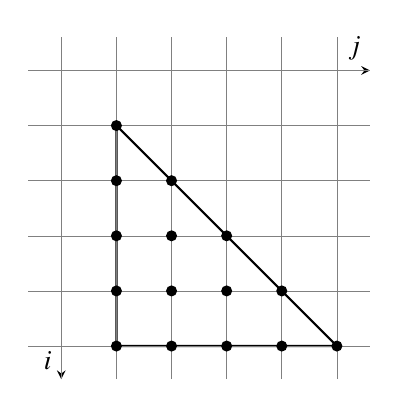
\begin{tikzpicture}[>=stealth,x=0.7cm,y=-0.7cm]
\draw[thick] (1,1)--(5,5)--(1,5)--(1,1);
\draw[->] (-0.6,0) to (5.6,0) node[anchor=south east] {$j$};
\draw[->] (0,-0.6) to (0,5.6) node[anchor=south east] {$i$};
\draw[help lines,step=0.7cm] (-0.6,5.6) grid (5.6,-0.6);
\foreach \i in {1,...,5}{
    \foreach \j in {1,...,\i}{
        \fill (\j,\i) circle (2pt);
    }
}
\end{tikzpicture}
\caption{The iteration domain of the loop nest in \autoref{f:loop nest}}
\label{f:iteration domain}
\end{figure}

Within the polyhedral model for analysis and transformation of
static affine programs, the most basic kind of set is the
\defindex{iteration domain}.
The iteration domain represents the iterations of a statement in a loop nest.
Take, for example, the loop nest in \autoref{f:loop nest}
and assume first that \lstinline{n} has a fixed value, say 5.
The pairs of values of \lstinline{i} and \lstinline{j} for
which statement \lstinline{S} is executed are shown graphically
in \autoref{f:iteration domain}.
Mathematically, this set of pairs can be represented as
$$
\{\,
(i,j) \in \ZZ^2 \mid 1 \le i \le 5 \wedge 1 \le j \le i
\,\}
$$
and the \isl/ notation is very similar:
\begin{lstlisting}[columns=flexible,escapechar=@,language=]{}
{ [i,j] : 1 <= i <= 5 and 1 <= j <= i }
\end{lstlisting}
In this notation,
the coordinates are separated by commas and enclosed in square
brackets.  This description of the space in which the set lives
is followed by a colon and the constraints on the coordinates.
Assuming the iterators are incremented by one in every iterations
of the loop, a lower and upper bound on each loop iterator
can be read off from the initialization and the test.
Note that in an \iscc/ set,
the coordinates are assumed to be integer by default.
For an iteration domain to be representable by such a set,
the iterators therefore need to be integers.

The constraints of a set need to be affine, i.e., linear plus constant term.
These affine constraint may be combined through conjunctions (\texttt{and}),
disjunctions (\texttt{or}), projections (\texttt{exists}) and
negations (\texttt{not}).
Note that the formula is immediately converted
into \indac{DNF}, so it may sometimes be more efficient
to construct a set from smaller sets by applying
basic operations such as intersection ({\tt *}),
union ({\tt +}) and difference ({\tt -}).
For example, the following square with its diagonal removed,
$$
\{\,
(i,j) \mid 0 \le i,j \le 10 \wedge \lnot (i = j)
\,\}
$$
can be constructed as
\begin{lstlisting}[columns=flexible,escapechar=@,language=]{}
{ [i,j] : 0 <= i,j <= 10 } - { [i,i] }
\end{lstlisting}
or as
\begin{lstlisting}[columns=flexible,escapechar=@,language=]{}
{ [i,j] : 0 <= i,j <= 10 and not (i = j) }
\end{lstlisting}
Note that an occurrence of a relational operator in a set description
may define several constraints, one for each pair of arguments.
The elements in a list of arguments are separated by a comma.
If there are no constraints on the coordinates, i.e., in case of
a universe set, the colon may be omitted as well.
For example
\begin{lstlisting}[columns=flexible,escapechar=@,language=]{}
{ [] }
\end{lstlisting}
represents the entire (unnamed) zero-dimensional space,
and should not be confused with
\begin{lstlisting}[columns=flexible,escapechar=@,language=]{}
{ }
\end{lstlisting}
which represents the empty set.

Returning to the iteration domain of the loop nest
in \autoref{f:loop nest}, we usually do not want to analyze
such a program for a specific value of \lstinline{n},
but instead for all possible values of \lstinline{n} at once.
A generic description of the iteration domain can be obtained
through the introduction of a (free) parameter, as in
\begin{lstlisting}[columns=flexible,escapechar=@,language=]{}
[n] -> { [i,j] : 1 <= i <= n and 1 <= j <= i }
\end{lstlisting}
The optional parameters should
be declared by placing them in a comma delimited list inside \lstinline![]!
(followed by an ``\lstinline!->!'') in front of the main set description.
The parameters are global and are identified by their names,
so the order inside the list is arbitrary.
This should be contrasted to the coordinates of a space, the names of
which are only relevant within the description of the set and which
are instead identified by their positions.
That is,
\begin{lstlisting}[columns=flexible,escapechar=@,language=]{}
[n] -> { [i,j] : 1 <= i <= n and 1 <= j <= i }
\end{lstlisting}
is equal to
\begin{lstlisting}[columns=flexible,escapechar=@,language=]{}
[n] -> { [a,b] : 1 <= a <= n and 1 <= b <= a }
\end{lstlisting}
but it is not equal to
\begin{lstlisting}[columns=flexible,escapechar=@,language=]{}
[n] -> { [j,i] : 1 <= i <= n and 1 <= j <= i }
\end{lstlisting}
(because the order of the coordinates has changed)
or
\begin{lstlisting}[columns=flexible,escapechar=@,language=]{}
[m] -> { [i,j] : 1 <= i <= m and 1 <= j <= i }
\end{lstlisting}
(because it involves a different parameter).

It is sometimes convenient to represent constraints that only
involve parameters and that are not tied to any particular space.
To construct such a parameter domain, the list of coordinates
should simply be omitted.  Note that the colon is required
in this case, even if there are no constraints.
In particular,
\begin{lstlisting}[columns=flexible,escapechar=@,language=]{}
{ : }
\end{lstlisting}
represents the universal parameter domain, which is very different
from the empty set.

To plug in a particular value for a parameter, the user should
take the \ai{intersection} (\ai[\tt]{*}) with a parameter domain
assigns a particular value to the parameter.
For example,
\begin{lstlisting}[columns=flexible,escapechar=@,language=]{}
S := [n] -> { [i,j] : 1 <= i <= n and 1 <= j <= i };
S * [n] -> { : n = 5 };
\end{lstlisting}
It should be noted, though, that the result is not the same
as simply replacing \lstinline{n} by 5 as the result of the above
sequence will still have the global parameter \lstinline{n} set to 5.
To avoid this assignment, the user should instead compute
the \ai{gist} (\ai[\tt]{\%}) of the original set in the context
of setting \lstinline{n} to 5.
That is, the result of the sequence below is \lstinline{True}.
\begin{lstlisting}[columns=flexible,escapechar=@,language=]{}
S1 := { [i,j] : 1 <= i <= 5 and 1 <= j <= i };
S2 := [n] -> { [i,j] : 1 <= i <= n and 1 <= j <= i };
(S2 % [n] -> { : n = 5}) = S1;
\end{lstlisting}

\begin{figure}
\begin{lstlisting}[escapechar=@]{}
for (i = 1; i <= n; i += 3)
    /* S */
\end{lstlisting}
\caption{A loop with non-unit stride}
\label{f:stride}
\end{figure}

If a loop has a non-unit stride as in \autoref{f:stride}
then affine constraints on the coordinates and the parameters
are not sufficient to represent the iteration domain.
What is needed is a way to express that the value of
\lstinline{i} is equal to 1 plus 3 times some integer and
this is where existentially quantified variables can be used.
Existentially quantified variables are introduced by the
\ai[\tt]{exists} keyword and followed by a colon.
They can only be used within a single disjunct.
As an example, the iteration domain of the loop in \autoref{f:stride}
can be represented as
\begin{lstlisting}[columns=flexible,escapechar=@,language=]{}
[n] -> { [i] : exists a : 1 <= i <= n and i = 1 + 3 a }
\end{lstlisting}

\begin{figure}
\begin{lstlisting}[escapechar=@]{}
for (i = 1; i <= n; ++i)
    if ((i + 1) % 5 <= 2)
	/* S */
\end{lstlisting}
\caption{A loop with a modulo condition}
\label{f:modulo}
\end{figure}

Existentially quantified variables are also useful to represent
modulo constraints.  Consider for example the loop in
\autoref{f:modulo}.  The iterator values \lstinline!i! for which
the statement \lstinline!S! is executed lie between
1 and \lstinline!n! and are such that the remainder of
\lstinline!i + 1! on division by 5 is less than or equal to 2.
The constraint $(i + 1) \bmod 5 \le 2$ can be written
as $(i + 1) - 5 \floor{\frac{i+1}5} \le 2$, where
$f = \floor{\frac{i+1}5}$ is the greatest integer part of $\frac{i+1}5$.
That is, $f$ is the unique integer value satisfying the constraints
$5 f \le i + 1$ and $5 f \ge (i+1) - 4$.
The iteration domain of the statement in \autoref{f:modulo}
can therefore be represented as
\begin{lstlisting}[columns=flexible,escapechar=@,language=]{}
[n] -> { [i] : exists f : 1 <= i <= n and (i + 1) - 5 f <= 2 and
	 (i + 1) - 4 <= 5 f <= i + 1 }
\end{lstlisting}
Since greatest integer parts occur relatively frequently, there is
a special notation for them in \isl/ using \lstinline![]!.
The above set can therefore also be represented as
\begin{lstlisting}[columns=flexible,escapechar=@,language=]{}
[n] -> { [i] : 1 <= i <= n and (i + 1) - 5 * [(i + 1)/5] <= 2 }
\end{lstlisting}
Actually, since modulos are pretty common too, \isl/ also has
a special notation for them and the set can therefore also be respresented as
\begin{lstlisting}[columns=flexible,escapechar=@,language=]{}
[n] -> { [i] : 1 <= i <= n and (i + 1) % 5 <= 2 }
\end{lstlisting}
It should be noted that \lstinline![]! always rounds down
(towards $-\infty$), while integer division in C truncates
(towards 0).  When translating conditions in C containing integer
divisions and/or modulos to \isl/ constraints, the user should therefore
make sure the sign of the dividend is positive.  If not, the integer
division needs to be translated differently for positive and negative
values.

\begin{figure}
\begin{lstlisting}[escapechar=@]{}
for (i = 0; i < n; ++i)
T:  t[i] = a[i];
for (i = 0; i < n; ++i)
    for (j = 0; j < n - i; ++j)
F:      t[j] = f(t[j], t[j+1]);
for (i = 0; i < n; ++i)
B:  b[i] = t[i];
\end{lstlisting}
\caption{A program with three loop nests}
\label{f:three loops}
\end{figure}

Most programs involve more than one statement.
Although it is possible to work with different sets, each
representing the iteration domain of a statement,
it is usually more convenient to collect all iteration domains
in a single set.  To be able to differentiate between iterations
of different statements with the same values for the iterators,
\isl/ allows spaces to be named.  The name is placed in front
of the \lstinline![]! enclosing the iterators.
Consider for example the program in \autoref{f:three loops}.
The program contains three statements which have been labeled
for convenience.
The iteration domain of the first statement (\lstinline!T!)
can be represented as
\begin{lstlisting}[columns=flexible,escapechar=@,language=]{}
[n] -> { T[i] : 0 <= i < n }
\end{lstlisting}
The union of all iteration domains can be represented as
\begin{lstlisting}[columns=flexible,escapechar=@,language=]{}
[n] -> {
    T[i] : 0 <= i < n;
    F[i,j] : 0 <= i < n and 0 <= j < n - i;
    B[i] : 0 <= i < n
}
\end{lstlisting}
The semicolon \lstinline{;} is used to express a disjunction
between spaces.  This should be contrasted with the \lstinline{or}
keyword which expresses a disjunction between conjunctions of constraints.
For example, the result of the following \iscc/ statement is
\lstinline{True}.
\begin{lstlisting}[columns=flexible,escapechar=@,language=]{}
{ [i] : i = 3 or i = 5 } = { [3]; [5] };
\end{lstlisting}

\subsubsection{Maps and Access Relations}

A second important concept in the polyhedral model is that
of an \defindex{access relation}.
An access relation connects iterations of a statement
to the array elements accessed by those iterations.
Such a binary relation can be represented by a map in \isl/.
Maps are defined in similar way to sets,
except that the single space is replaced by a pair of spaces separated
by \verb!->!.
As an example, consider once more the program in \autoref{f:three loops}.
In particular, consider the access \lstinline{t[j+1]} in
statement \lstinline{F}.
The index expression maps the pair of iterations \lstinline{i}
and \lstinline{j} to \lstinline{t[j+1]}, i.e., element \lstinline{j+1}
of a space with name \lstinline{t}.
Ignoring the loop bound constraints, this access relation can
be represented as
\begin{lstlisting}[columns=flexible,escapechar=@,language=]{}
{ F[i,j] -> t[j + 1] }
\end{lstlisting}
It is however customary to include the constraints on the iterators
in the access relation, resulting in
\begin{lstlisting}[columns=flexible,escapechar=@,language=]{}
[n] -> { F[i,j] -> t[j + 1] : 0 <= i < n and 0 <= j < n - i }
\end{lstlisting}
The constraints can be added by intersecting the domains
of the access relations with the iteration domains.
For example, the following sequence constructs the access
relation for all reads in the program.
\begin{lstlisting}[columns=flexible,escapechar=@,language=]{}
D := [n] -> {
    T[i] : 0 <= i < n;
    F[i,j] : 0 <= i < n and 0 <= j < n - i;
    B[i] : 0 <= i < n
};
Read := {
    T[i] -> a[i];
    F[i,j] -> t[j];
    F[i,j] -> t[j + 1];
    B[i] -> t[i]
};
Read := Read * D;
\end{lstlisting}
In this sequence, the \lstinline{*} operator, when applied
to a map and a set, intersects the domain of the map with the set.

The notation \lstinline{R(S)} can be used to compute the image
of the set \lstinline{S} under the map \lstinline{R}.
For example, given the sequence above, \lstinline!Read({F[0,1]})!
computes the array elements read in iteration $(0,1)$ of statement
\lstinline{F} and is equal to
\begin{lstlisting}[columns=flexible,escapechar=@,language=]{}
[n] -> { t[2] : n >= 2; t[1] : n >= 2 }
\end{lstlisting}
That is, elements 1 and 2 of the \lstinline{t} array are read,
provided \lstinline{n} is at least 2.

Maps need not be single-valued.
As an example, assume that \lstinline{A} is a two-dimensional
array of size \lstinline{n} in both dimensions.
Iterations \lstinline{i} of
a statement \lstinline{S} may pass a pointer to an entire row
of \lstinline{A} to a function as in \lstinline{f(A[i])}.
Without knowing anything about \lstinline{f}, we would have
to assume that this function may access any element of the row.
The access relation corresponding to \lstinline{A[i]} is therefore
\begin{lstlisting}[columns=flexible,escapechar=@,language=]{}
[n] -> { S[i] -> A[i,j] : 0 <= i,j < n }
\end{lstlisting}
This map associates \lstinline{n} elements of \lstinline{A}
to each iteration of \lstinline{S}.

\subsubsection{Nested Spaces}

Each space may contain a nested pair of spaces.  Such nested spaces
are extremely useful in more advanced applications.
As an example, suppose that during equivalence checking
\shortcite{Verdoolaege2009equivalence}
of two programs the iterations of \verb!S1! in one program are supposed to
produce the same results as the same iterations of \verb!SA! in the other program,
which may be described using the following map
\begin{verbatim}
[n] -> { S1[i] -> SA[i] : 0 <= i <= n }
\end{verbatim}
If the iterations of \verb!S1! depend on the same iterations
of \verb!S2!, i.e., \verb!{S1[i]->S2[i]}!, while those of \verb!SA!
depend on the next iteration of \verb!B!, i.e., \verb!{SA[i]->SB[i+1]}!,
then we can apply the cross product of these two dependence maps, i.e.,
\begin{verbatim}
{ [S1[i] -> SA[i']] -> [S2[i] -> SB[1+i']] }
\end{verbatim}
to the original map to find
out which iterations of \verb!S2! should correspond to which
iterations of \verb!SB!.

\subsubsection{Basic Operations}

Basic operations on sets and maps include intersection (\ai[\tt]{*}),
union (\ai[\tt]{+}), difference (\ai[\tt]{-}), cross product (\ai[\tt]{cross}),
sampling (\ai[\tt]{sample}), affine hull (\ai[\tt]{aff}),
lexicographic optimization (\ai[\tt]{lexmin} or \ai[\tt]{lexmax}),
subset (\ai[\tt]{<=}) and equality (\ai[\tt]{=}) tests,
code generation (\ai[\tt]{codegen})
and the cardinality (\ai[\tt]{card}).
Additional operations on maps include computing domain (\ai[\tt]{dom})
and range (\ai[\tt]{ran}), differences between image and domain (\ai[\tt]{deltas}),
join (\ai[\tt]{.}), inverse (\ai[\tt]{\^{}-1}) and transitive closure (\ai[\tt]{\^{}+}).
The latter may result in an overapproximation.

The \ai[\tt]{card} operation computes the number of elements in a set
or the number of elements in the image of a domain element of a map.
The operation is performed exactly and completely symbolically and
the result is a piecewise quasipolynomial, i.e., a subdivision of one
or more spaces, with a quasipolynomial associated to each cell in the subdivision.
As a trivial example, the result of
\begin{verbatim}
card { A[i] -> B[j] : 0 <= j <= i }
\end{verbatim}
is \verb!{ A[i] -> (1+i) : i >= 0 }!.
Operations on piecewise quasipolynomials include sum (\ai[\tt]{+})
and difference (\ai[\tt]{-}) and the computation of an upper bound over the domain.
If the domain contains a pair of nested spaces, then the upper bound is computed over
the nested range.  As another trivial example, the result of
\begin{verbatim}
ub{ [[i] -> [j]] -> j^2 : -i <= j <= i }
\end{verbatim}
is
\verb!({ [i] -> max(i^2) : i >= 0 }, True)!.
The first element in this list is the actual bound in the form
of a piecewise quasipolynomial fold,
i.e., a maximum of quasipolynomials defined over cells.
The second indicates whether the bound is tight, i.e., whether
a maximum has been computed.

\subsubsection{Advanced Operations}

While the basic {\tt card} operation simply counts the number of elements
in an affine set, it is also possible to assign a weight to each element
of the set and to compute the sum of those weights over all the points in the set.
The syntax for this weighted counting is to compute the {\tt sum} of
a piecewise quasipolynomial over its domain.  As in the case of the {\tt ub}
operator, if the domain contains a pair of nested space, the sum is computed
over the range.  As an example, the result
of
\begin{verbatim}
sum{ [[i] -> [j]] -> i*j : 0 <= j <= i }
\end{verbatim}
is
\verb|{ [i] -> (1/2*i^2+1/2*i^3) : i >= 0 }|.

After the computation of some sum or bound, the result may have to
be reformulated in terms of other variables.  For example, during
inter procedural analysis, a result computed in terms of the formal
parameters may have to be reformulated in terms of the actual parameters.
{\tt iscc} therefore allows maps and
piecewise quasipolynomials or folds to be composed.
If the map is multi-valued, then the composition maps each domain element
to the sum or upper bound of the values at its image elements.

Finally, because of its high-level representation, {\tt iscc} can
provide a dependence analysis operation taking only three maps as input,
the sink accesses, the potential source accesses and a schedule.
The result is a single dependence map.


\subsubsection{More Examples}
\begin{verbatim}
P := [n, m] -> { [i,j] : 0 <= i <= n and i <= j <= m };
card P;

f := [n,m] -> { [i,j] -> i*j + n*i*i*j : i,j >= 0 and 5i + 27j <= n+m };
sum f;
s := sum f;
s @ [n,m] -> { : 0 <= n,m <= 20 };

f := [n] -> { [i] -> 2*n*i - n*n + 3*n - 1/2*i*i - 3/2*i-1 :
                (exists j : 0 <= i < 4*n-1 and 0 <= j < n and
                            2*n-1 <= i+j <= 4*n-2 and i <= 2*n-1 ) };
ub f;
u := (ub f)[0];
u @ [n] -> { : 0 <= n <= 10 };

m := [n] -> { [i,j] -> [i+1,j+1] : 1 <= i,j < n;
              [i,j] -> [i+1,j-1] : 1 <= i < n and 2 <= j <= n };
m^+;
(m^+)[0];

codegen [N] -> { A[i] -> [i,0] : 0 <= i <= N; B[i] -> [i,1] : 1 <= i <= N };

{ [k] -> [i] : 1 <= i <= k } . { [n] -> 2 * n : n >= 1 };

{ [m] -> [c] : 1 <= c <= m } . { [k] -> max((3 * k + k^2)) : k >= 1 };
\end{verbatim}

\subsubsection{Comparison to other Interactive Polyhedral Tools}

Two related interactive polyhedral tools are
the Omega calculator \shortcite{Omega_calc}
and {\tt SPPoC} \shortcite{Boulet2001SPPoC}.
The syntax of {\tt iscc} was very much inspired
by that of the Omega calculator.  However, the Omega
calculator only knows sets and maps.  In particular,
it does not perform any form of counting.  An earlier version
of \barvinok/ came with a modified version of
the Omega calculator that introduced an operation
for counting the number of elements in a set, but it
would simply print the result and not allow any further
manipulations.
{\tt SPPoC} does support counting, but only the basic
operation of counting the elements in a set.
In particular, it does not support weighted counting,
nor the computation of upper bounds.
It also only supports (single-valued) functions
and not generic relations like the Omega calculator and {\tt iscc}.
Internally, {\tt SPPoC} uses {\tt PolyLib}, {\tt PipLib} and {\tt omega}
to perform
its operations.  Although the first two of these libraries may have been
state-of-the-art at the time {\tt SPPoC} was created, they are
no longer actively maintained and have been largely
superseded by more recent libraries.
In particular, {\tt PipLib} effectively only supports a single
operation, which is now also available in both {\tt isl} and {\tt PPL}.
The operations on rational polyhedra in {\tt PolyLib} are also
available in {\tt PPL}, usually through a cleaner interface and
with a more efficient implementation.  As to counting the elements
in a parametric polytope, Barvinok's algorithm,
implemented in the {\tt barvinok} library, is usually much faster
than the algorithm implemented in {\tt PolyLib}
\shortcite{Verdoolaege2007parametric}.
Furthermore,
the ability to work with named and nested spaces and the ability
of sets and maps to contain (pairs of) elements from different spaces
are not available in the Omega calculator and {\tt SPPoC}.

\newpage
\tablecaption{{\tt iscc} operations.  The variables
have the following types,
$s$: set,
$m$: map,
$q$: piecewise quasipolynomial,
$f$: piecewise quasipolynomial fold,
$t$: schedule (tree),
$l$: list,
$i$: integer,
$b$: boolean,
$S$: string,
$o$: object of any type
}
\label{t:iscc}
\tablehead{
\hline
Syntax & Meaning
\\
\hline
}
\tabletail{
\multicolumn{2}{r}{\small\sl continued on next page}
\\
}
\tablelasttail{}
\begin{supertabular}{p{0.35\textwidth}p{0.6\textwidth}}
$s_2$ := \ai[\tt]{aff} $s_1$ & affine hull of $s_1$
\\
$m_2$ := \ai[\tt]{aff} $m_1$ & affine hull of $m_1$
\\
$q$ := \ai[\tt]{card} $s$ &
number of elements in the set $s$
\\
$q$ := \ai[\tt]{card} $m$ &
number of elements in the image of a domain element
\\
$s_2$ := \ai[\tt]{coalesce} $s_1$ &
simplify the representation of set $s_1$ by trying
to combine pairs of basic sets into a single
basic set
\\
$m_2$ := \ai[\tt]{coalesce} $m_1$ &
simplify the representation of map $m_1$ by trying
to combine pairs of basic maps into a single
basic map
\\
$q_2$ := \ai[\tt]{coalesce} $q_1$ &
simplify the representation of $q_1$ by trying
to combine pairs of basic sets in the domain
of $q_1$ into a single basic set
\\
$f_2$ := \ai[\tt]{coalesce} $f_1$ &
simplify the representation of $f_1$ by trying
to combine pairs of basic sets in the domain
of $f_1$ into a single basic set
\\
\ai[\tt]{codegen} $t$ &
generate code for the given schedule.
\\
\ai[\tt]{codegen} $m$ &
generate code for the given schedule.
\\
\ai[\tt]{codegen} $m_1$ \ai[\tt]{using} $m_2$ &
generate code for the schedule $m_1$ using the options $m_2$.
\\
$s_2$ := \ai[\tt]{coefficients} $s_1$ &
The set of coefficients of valid constraints for $s_1$
\\
$s_2$ := \ai[\tt]{solutions} $s_1$ &
The set of elements satisfying the constraints with coefficients in $s_1$
\\
$s_3$ := $s_1$ \ai[\tt]{cross} $s_2$ &
Cartesian product of $s_1$ and $s_2$
\\
$m_3$ := $m_1$ \ai[\tt]{cross} $m_2$ &
Cartesian product of $m_1$ and $m_2$
\\
$m_3$ := $m_1$ \ai[\tt]{cross\_range} $m_2$ &
Cartesian product of the ranges of $m_1$ and $m_2$ for their shared domain
\\
$s$ := \ai[\tt]{deltas} $m$ &
the set $\{\, y - x \mid x \to y \in m \,\}$
\\
$m_2$ := \ai[\tt]{deltas\_map} $m_1$ &
the map $\{\, (x \to y) \to y - x \mid x \to y \in m_1 \,\}$
\\
$s$ := \ai[\tt]{dom} $m$ &
domain of map $m$
\\
$s$ := \ai[\tt]{dom} $q$ &
domain of piecewise quasipolynomial $q$
\\
$s$ := \ai[\tt]{dom} $f$ &
domain of piecewise quasipolynomial fold $f$
\\
$s$ := \ai[\tt]{dom} $t$ &
domain of schedule $t$
\\
$s$ := \ai[\tt]{domain} $m$ &
domain of map $m$
\\
$s$ := \ai[\tt]{domain} $q$ &
domain of piecewise quasipolynomial $q$
\\
$s$ := \ai[\tt]{domain} $f$ &
domain of piecewise quasipolynomial fold $f$
\\
$s$ := \ai[\tt]{domain} $t$ &
domain of schedule $t$
\\
$m_2$ := \ai[\tt]{domain\_map} $m_1$ &
a map from a wrapped copy of $m_1$ to the domain of $m_1$
\\
$s$ := \ai[\tt]{ran} $m$ &
range of map $m$
\\
$s$ := \ai[\tt]{range} $m$ &
range of map $m$
\\
$m_2$ := \ai[\tt]{range\_map} $m_1$ &
a map from a wrapped copy of $m_1$ to the range of $m_1$
\\
$m$ := \ai[\tt]{identity} $s$ &
identity relation on $s$
\\
$q$ := \ai[\tt]{lattice\_width} $s$ &
lattice width of the set $s$
\\
$l$ := \ai[\tt]{lb} $q$ &
compute a
lower bound on the piecewise quasipolynomial $q$ over
all integer points in the domain of $q$
and return a list containing the lower bound
and a boolean that is true if the lower bound
is known to be tight.
If the domain of $q$ wraps a map, then the lower
bound is computed over all integer points in
the range of the wrapped map instead.
\\
$s_2$ := \ai[\tt]{lexmin} $s_1$ &
lexicographically minimal element of $s_1$
\\
$m_2$ := \ai[\tt]{lexmin} $m_1$ &
lexicographically minimal image element
\\
$s_2$ := \ai[\tt]{lexmax} $s_1$ &
lexicographically maximal element of $s_1$
\\
$m_2$ := \ai[\tt]{lexmax} $m_1$ &
lexicographically maximal image element
\\
$s_2$ := \ai[\tt]{lift} $s_1$ &
lift $s_1$ to a space with extra dimensions corresponding
to the existentially quantified variables in $s_1$ such
that \lstinline!domain(unwrap(lift S))! is equal to \lstinline!S!
\\
$m$ := \ai[\tt]{map} $t$ &
convert schedule $t$ to a map representation
\\
$s_2$ := \ai[\tt]{params} $s_1$ &
parameter domain of set $s_1$
\\
$s$ := \ai[\tt]{params} $m$ &
parameter domain of map $m$
\\
$l$ := \ai[\tt]{parse\_file} $S$ &
parse the file names $S$ and return a list consisting of
the iteration domain, the must write access relation,
the may write access relation, the read access relation and
the original schedule.
This operation is only available if \ai[\tt]{pet}
support was compiled in.
\\
$s_2$ := \ai[\tt]{poly} $s_1$ & polyhedral hull of $s_1$
\\
$m_2$ := \ai[\tt]{poly} $m_1$ & polyhedral hull of $m_1$
\\
$q_2$ := \ai[\tt]{poly} $q_1$ & polynomial approximation of $q_1$
\\
$q_2$ := \ai[\tt]{lpoly} $q_1$ & polynomial underapproximation of $q_1$
\\
$q_2$ := \ai[\tt]{upoly} $q_1$ & polynomial overapproximation of $q_1$
\\
$l$ := \ai[\tt]{pow} $m$\ &
compute an overapproximation of the power
of $m$ and return a list containing the overapproximation
and a boolean that is true if the overapproximation
is known to be exact
\\
\ai[\tt]{print} $o$ &
print object
\\
$o$ := \ai[\tt]{read} {\tt "}{\it filename}{\tt"} &
read object from file
\\
$s_2$ := \ai[\tt]{sample} $s_1$ &
a sample element of the set $s_1$
\\
$m_2$ := \ai[\tt]{sample} $m_1$ &
a sample element of the map $m_1$
\\
$s_2$ := \ai[\tt]{scan} $s_1$ &
the set $s_1$ split into individual elements,
provided $s_1$ contains a finite number of elements
\\
$m_2$ := \ai[\tt]{scan} $m_1$ &
the map $m_1$ split into individual elements,
provided $m_1$ contains a finite number of elements
\\
\ai[\tt]{source} {\tt "}{\it filename}{\tt"} &
read commands from file
\\
$q_2$ := \ai[\tt]{sum} $q_1$ &
sum $q_1$ over all integer points in the domain of $q_1$,
or, if the domain of $q_1$ wraps a map, over all integer
points in the range of the wrapped map.
\\
$S$ := \ai[\tt]{typeof} $o$ &
a string representation of the type of $o$
\\
$l$ := \ai[\tt]{ub} $q$ &
compute an
upper bound on the piecewise quasipolynomial $q$ over
all integer points in the domain of $q$
and return a list containing the upper bound
and a boolean that is true if the upper bound
is known to be tight.
If the domain of $q$ wraps a map, then the upper
bound is computed over all integer points in
the range of the wrapped map instead.
\\
$l$ := \ai[\tt]{vertices} $s$ &
a list of vertices of the rational polytope defined by the same constraints
as $s$
\\
$s$ := \ai[\tt]{wrap} $m$ &
wrap the map in a set
\\
$m$ := \ai[\tt]{unwrap} $s$ &
unwrap the map from the set
\\
\ai[\tt]{write} {\tt "}{\it filename}{\tt"} $o$ &
write object to file
\\
$m_2$ := \ai[\tt]{zip} $m_1$ &
the cross product of domain and range of $m_1$, i.e.,
$\{\, (\vec w \to \vec y) \to (\vec x \to \vec z)
\mid (\vec w \to \vec x) \to (\vec y \to \vec z) \in m_1 \,\}$
\\
$m_3$ := \ai[\tt]{any} $m_1$ \ai[\tt]{before} $m_2$ \ai[\tt]{under} $t$ &
compute a map from any element $x$ in the domain of $m_1$
to any element $y$ in the domain of $m_2$
such that their images $m_1(x)$ and $m_2(y)$ overlap
and such that $x$ is scheduled before $y$ by $t$.
\\
$m_4$ := \ai[\tt]{any} $m_1$ \ai[\tt]{before} $m_2$ \ai[\tt]{under} $m_3$ &
same as the previous operation, with the schedule represented by a map.
\\
$l$ := \ai[\tt]{last} $m_1$ \ai[\tt]{before} $m_2$ \ai[\tt]{under} $t$ &
compute a map that contains for any element $y$ in the domain of $m_2$
a mapping from the last element $x$ in the domain of $m_1$
(according to the schedule $t$) to $y$
such that $m_1(x)$ and $m_2(y)$ overlap
and such that $x$ is scheduled before $y$ by $t$.
Return a list containing this map and the subset of
$m_2$ for which there is no corresponding element in the domain of $m_1$.
\\
$l$ := \ai[\tt]{last} $m_1$ \ai[\tt]{before} $m_2$ \ai[\tt]{under} $m_3$ &
same as the previous operation, with the schedule represented by a map.
\\
$m_4$ := \ai[\tt]{any} $m_1$ \ai[\tt]{last} $m_2$ \ai[\tt]{before} $m_3$
\ai[\tt]{under} $t$ &
compute a map that contains for any element $y$ in the domain of $m_3$
a mapping from the last element $x$ in the domain of $m_2$
(according to the schedule $t$) to $y$
such that $m_2(x)$ and $m_3(y)$ overlap
and such that $x$ is scheduled before $y$ by $t$
as well as from any element $z$ in the domain of $m_1$ such that
$m_1(z)$ and $m_3(y)$ overlap,
$z$ is scheduled before $y$ by $t$
and such that there is no $x$ in the domain of $m_2$ with
$m_2(x) \cap m_3(y) \ne \emptyset$ and
$x$ scheduled between $z$ and $y$ by $t$.
\\
$m_5$ := \ai[\tt]{any} $m_1$ \ai[\tt]{last} $m_2$ \ai[\tt]{before} $m_3$
\ai[\tt]{under} $m_4$ &
same as the previous operation, with the schedule represented by a map.
\\
$t$ := \ai[\tt]{schedule} $s$ \ai[\tt]{respecting} $m_1$ \ai[\tt]{minimizing} $m_2$ &
compute a schedule for the domains in $s$ that respects all dependences
in $m_1$ and tries to minimize the dependences in $m_2$.
\\
$b_3$ := $b_1$ \ai{$+$} $b_2$ & or
\\
$i_3$ := $i_1$ \ai{$+$} $i_2$ & sum
\\
$s_3$ := $s_1$ \ai{$+$} $s_2$ & union
\\
$m_3$ := $m_1$ \ai{$+$} $m_2$ & union
\\
$q_3$ := $q_1$ \ai{$+$} $q_2$ & sum
\\
$f_2$ := $f_1$ \ai{$+$} $q$ & sum
\\
$f_2$ := $q$ \ai{$+$} $f_1$ & sum
\\
$S_3$ := $S_1$ \ai{$+$} $S_2$ & concatenation
\\
$S_2$ := $o$ \ai{$+$} $S_1$ &
concatenation of stringification of $o$ and $S_1$
\\
$S_2$ := $S_1$ \ai{$+$} $o$ &
concatenation of $S_1$ and stringification of $o$
\\
$i_3$ := $i_1$ \ai{$-$} $i_2$ & difference
\\
$s_3$ := $s_1$ \ai{$-$} $s_2$ & set difference
\\
$m_3$ := $m_1$ \ai{$-$} $m_2$ & set difference
\\
$m_2$ := $m_1$ \ai{$-$} $s$ & subtract $s$ from the domain of $m_1$
\\
$m_2$ := $m_1$ \ai[\tt]{->-} $s$ & subtract $s$ from the range of $m_1$
\\
$q_3$ := $q_1$ \ai{$-$} $q_2$ & difference
\\
$b_3$ := $b_1$ \ai{$*$} $b_2$ & and
\\
$i_3$ := $i_1$ \ai{$*$} $i_2$ & product
\\
$s_3$ := $s_1$ \ai{$*$} $s_2$ & intersection
\\
$m_3$ := $m_1$ \ai{$*$} $m_2$ & intersection
\\
$q_2$ := $i$ \ai{$*$} $q_1$ & product
\\
$q_2$ := $q_1$ \ai{$*$} $i$ & product
\\
$q_3$ := $q_1$ \ai{$*$} $q_2$ & product
\\
$f_2$ := $i$ \ai{$*$} $f_1$ & product
\\
$f_2$ := $f_1$ \ai{$*$} $i$ & product
\\
$m_2$ := $m_1$ \ai{$*$} $s$ & intersect domain of $m_1$ with $s$
\\
$q_2$ := $q_1$ \ai{$*$} $s$ & intersect domain of $q_1$ with $s$
\\
$f_2$ := $f_1$ \ai{$*$} $s$ & intersect domain of $f_1$ with $s$
\\
$m_2$ := $m_1$ \ai[\tt]{->$*$} $s$ & intersect range of $m_1$ with $s$
\\
$s_2$ := $m$($s_1$) & apply map $m$ to set $s_1$
\\
$q_2$ := $q_1$($s$) & apply $q_1$ to each element in $s$ and compute
the sum of the results
\\
$l$ := $f$($s$) & apply $f$ to each element in $s$, compute
a bound of the results
and return a list containing the bound
and a boolean that is true if the bound
is known to be tight.
\\
$m_3$ := $m_1$ \ai[\tt]{.} $m_2$ & join of $m_1$ and $m_2$
\\
$m_3$ := $m_1$ \ai[\tt]{before} $m_2$ & join of $m_1$ and $m_2$
\\
$m_3$ := $m_2$($m_1)$ & join of $m_1$ and $m_2$
\\
$m_3$ := $m_2$ \ai[\tt]{after} $m_1$ & join of $m_1$ and $m_2$
\\
$f_3$ := $f_1$ \ai[\tt]{.} $f_2$ & join of $f_1$ and $f_2$, combining
the lists of quasipolynomials over shared domains
\\
$q_2$ := $m$ \ai[\tt]{.} $q_1$ & join of $m$ and $q_1$, taking the sum
over all elements in the intersection of the range of $m$ and the domain
of $q_1$
\\
$q_2$ := $m$ \ai[\tt]{before} $q_1$ & $q_2$ := $m$ \ai[\tt]{.} $q_1$
\\
$q_2$ := $q_1(m)$ & $q_2$ := $m$ \ai[\tt]{.} $q_1$
\\
$q_2$ := $q_1$ \ai[\tt]{after} $m$ & $q_2$ := $m$ \ai[\tt]{.} $q_1$
\\
$l$ := $m$ \ai[\tt]{.} $f$ & join of $m$ and $f$, computing a bound
over all elements in the intersection of the range of $m$ and the domain
of $f$ and returning a list containing the bound
and a boolean that is true if the bound is known to be tight.
\\
$l$ := $m$ \ai[\tt]{before} $f$ & $l$ := $m$ \ai[\tt]{.} $f$
\\
$l$ := $f(m)$ & $l$ := $m$ \ai[\tt]{.} $f$
\\
$l$ := $f$ \ai[\tt]{after} $m$ & $l$ := $m$ \ai[\tt]{.} $f$
\\
$m$ := $s_1$ \ai[\tt]{->} $s_2$ & universal map with domain $s_1$
and range $s_2$
\\
$q_2$ := $q_1$ \ai{@} $s$ &
evaluate the piecewise quasipolynomial $q_1$ in each element
of the set $s$ and return a piecewise quasipolynomial
mapping each of the individual elements to the resulting
constant
\\
$q$ := $f$ \ai{@} $s$ &
evaluate the piecewise quasipolynomial fold $f$ in each element
of the set $s$ and return a piecewise quasipolynomial
mapping each of the individual elements to the resulting
constant
\\
$s_3$ := $s_1$ \ai[\tt]{\%} $s_2$ &
simplify $s_1$ in the context of $s_2$, i.e., compute
the gist of $s_1$ given $s_2$
\\
$m_3$ := $m_1$ \ai[\tt]{\%} $m_2$ &
simplify $m_1$ in the context of $m_2$, i.e., compute
the gist of $m_1$ given $m_2$
\\
$m_2$ := $m_1$ \ai[\tt]{\%} $s$ &
simplify $m_1$ in the context of the domain $s$, i.e., compute
the gist of $m_1$ given domain $s$
\\
$q_2$ := $q_1$ \ai[\tt]{\%} $s$ &
simplify $q_1$ in the context of the domain $s$, i.e., compute
the gist of $q_1$ given $s$
\\
$f_2$ := $f_1$ \ai[\tt]{\%} $s$ &
simplify $f_1$ in the context of the domain $s$, i.e., compute
the gist of $f_1$ given $s$
\\
$m_2$ := $m_1$\ai[\tt]{\^{}}i & the $i$th power of $m_1$;
if $i$ is negative then the result is the ($-i$)th power of the inverse
of $m_1$
\\
$l$ := $m$\ai[\tt]{\^{}+} &
compute an overapproximation of the transitive closure
of $m$ and return a list containing the overapproximation
and a boolean that is true if the overapproximation
is known to be exact
\\
$o$ := $l$[$i$] &
the element at position $i$ in the list $l$
\\
$b$ := $q_1$ \ai[\tt]{==} $q_2$ & is $q_1$ obviously equal to $q_2$?
\\
$b$ := $f_1$ \ai[\tt]{==} $f_2$ & is $f_1$ obviously equal to $f_2$?
\\
$b$ := $s_1$ \ai[\tt]{=} $s_2$ & is $s_1$ equal to $s_2$?
\\
$b$ := $m_1$ \ai[\tt]{=} $m_2$ & is $m_1$ equal to $m_2$?
\\
$b$ := $S_1$ \ai[\tt]{=} $S_2$ & is $S_1$ equal to $S_2$?
\\
$b$ := $s_1$ \ai[\tt]{<=} $s_2$ & is $s_1$ a subset of $s_2$?
\\
$b$ := $m_1$ \ai[\tt]{<=} $m_2$ & is $m_1$ a subset of $m_2$?
\\
$b$ := $s_1$ \ai[\tt]{<} $s_2$ & is $s_1$ a proper subset of $s_2$?
\\
$b$ := $m_1$ \ai[\tt]{<} $m_2$ & is $m_1$ a proper subset of $m_2$?
\\
$b$ := $s_1$ \ai[\tt]{>=} $s_2$ & is $s_1$ a superset of $s_2$?
\\
$b$ := $m_1$ \ai[\tt]{>=} $m_2$ & is $m_1$ a superset of $m_2$?
\\
$b$ := $s_1$ \ai[\tt]{>} $s_2$ & is $s_1$ a proper superset of $s_2$?
\\
$b$ := $m_1$ \ai[\tt]{>} $m_2$ & is $m_1$ a proper superset of $m_2$?
\\
$m$ := $s_1$ \ai[\tt]{<<} $s_2$ & a map from
$s_1$ to $s_2$ of those elements that live in the same space and
such that the elements of $s_1$ are lexicographically strictly smaller
than those of $s_2$.
\\
$m_3$ := $m_1$ \ai[\tt]{<<} $m_2$ & a map from the domain of
$m_1$ to the domain of $m_2$ of those elements such that their images
live in the same space and such that the images of the elements of
$m_1$ are lexicographically strictly smaller than those of $m_2$.
\\
$m$ := $s_1$ \ai[\tt]{<<=} $s_2$ & a map from
$s_1$ to $s_2$ of those elements that live in the same space and
such that the elements of $s_1$ are lexicographically smaller
than those of $s_2$.
\\
$m_3$ := $m_1$ \ai[\tt]{<<=} $m_2$ & a map from the domain of
$m_1$ to the domain of $m_2$ of those elements such that their images
live in the same space and such that the images of the elements of
$m_1$ are lexicographically smaller than those of $m_2$.
\\
$m$ := $s_1$ \ai[\tt]{>>} $s_2$ & a map from
$s_1$ to $s_2$ of those elements that live in the same space and
such that the elements of $s_1$ are lexicographically strictly greater
than those of $s_2$.
\\
$m_3$ := $m_1$ \ai[\tt]{>>} $m_2$ & a map from the domain of
$m_1$ to the domain of $m_2$ of those elements such that their images
live in the same space and such that the images of the elements of
$m_1$ are lexicographically strictly greater than those of $m_2$.
\\
$m$ := $s_1$ \ai[\tt]{>>=} $s_2$ & a map from
$s_1$ to $s_2$ of those elements that live in the same space and
such that the elements of $s_1$ are lexicographically greater
than those of $s_2$.
\\
$m_3$ := $m_1$ \ai[\tt]{>>=} $m_2$ & a map from the domain of
$m_1$ to the domain of $m_2$ of those elements such that their images
live in the same space and such that the images of the elements of
$m_1$ are lexicographically greater than those of $m_2$.
\\
\end{supertabular}


\section{\protect\PolyLib/ interface of the \protect\ai[\tt]{barvinok} library
(obsolescent)}

Although \barvinok/ currently still uses \PolyLib/ internally,
this is likely to change in the not too distant future.
Consider using \isl/ based alternatives for the functions in this section
as the latter are likely to be removed in future releases.

Our \barvinok/ library is built on top of \PolyLib/ 
\shortcite{Wilde1993,Loechner1999}.
In particular, it reuses the implementations
of the algorithm of 
\shortciteN{Loechner97parameterized}
for computing parametric vertices
and the algorithm of
\shortciteN{Clauss1998parametric}
for computing chamber decompositions.
Initially, our library was meant to be a replacement
for the algorithm of \shortciteN{Clauss1998parametric},
also implemented in \PolyLib/, for computing quasi-polynomials.
To ease the transition of application programs we
tried to reuse the existing data structures as much as possible.

\subsection{Existing Data Structures}
\label{a:existing}

Inside \PolyLib/ integer values are represented by the 
\ai[\tt]{Value} data type.
Depending on a configure option, the data type may
either by a 32-bit integer, a 64-bit integer
or an arbitrary precision integer using \ai[\tt]{GMP}.
The \barvinok/ library requires that \PolyLib/ is compiled
with support for arbitrary precision integers.

The basic structure for representing (unions of) polyhedra is a
\ai[\tt]{Polyhedron}.
\begin{verbatim}
typedef struct polyhedron {
  unsigned Dimension, NbConstraints, NbRays, NbEq, NbBid;
  Value **Constraint;
  Value **Ray;
  Value *p_Init;
  int p_Init_size;
  struct polyhedron *next;
} Polyhedron;
\end{verbatim}
The attribute \ai[\tt]{Dimension} is the dimension
of the ambient space, i.e., the number of variables.
The attributes \ai[\tt]{Constraint}
and \ai[\tt]{Ray} point to two-dimensional arrays
of constraints and generators, respectively.
The number of rows is stored in
\ai[\tt]{NbConstraints} and
\ai[\tt]{NbRays}, respectively.
The number of columns in both arrays is equal
to \verb!1+Dimension+1!.
The first column of \ai[\tt]{Constraint} is either
$0$ or $1$ depending on whether the constraint 
is an equality ($0$) or an inequality ($1$).
The number of equalities is stored in \ai[\tt]{NbEq}.
If the constraint is $\sp a x + c \ge 0$, then
the next columns contain the coefficients $a_i$
and the final column contains the constant $c$.
The first column of \ai[\tt]{Ray} is either
$0$ or $1$ depending on whether the generator 
is a line ($0$) or a vertex or ray ($1$).
The number of lines is stored in \ai[\tt]{NbBid}.
Let $d$ be the \ac{lcm} of the denominators of the coordinates
of a vertex $\vec v$, then the next columns contain
$d v_i$ and the final column contains $d$.
For a ray, the final column contains $0$.
The field \ai[\tt]{next} points to the next polyhedron in
the union of polyhedra.
It is \verb+0+ if this is the last (or only) polyhedron in the union.
For more information on this structure, we refer to \shortciteN{Wilde1993}.

Quasi-polynomials are represented using the 
\ai[\tt]{evalue} and \ai[\tt]{enode} structures.
\begin{verbatim}
typedef enum { polynomial, periodic, evector } enode_type;

typedef struct _evalue {
  Value d;              /* denominator */
  union {
    Value n;            /* numerator (if denominator != 0) */
    struct _enode *p;   /* pointer   (if denominator == 0) */
  } x;
} evalue;

typedef struct _enode {
  enode_type type;      /* polynomial or periodic or evector */
  int size;             /* number of attached pointers */
  int pos;              /* parameter position */
  evalue arr[1];        /* array of rational/pointer */
} enode;
\end{verbatim}
If the field \ai[\tt]{d} of an \ai[\tt]{evalue} is zero, then
the \ai[\tt]{evalue} is a placeholder for a pointer to
an \ai[\tt]{enode}, stored in \ai[\tt]{x.p}.
Otherwise, the \ai[\tt]{evalue} is a rational number with
numerator \ai[\tt]{x.n} and denominator \ai[\tt]{d}.
An \ai[\tt]{enode} is either a \ai[\tt]{polynomial}
or a \ai[\tt]{periodic}, depending on the value
of \ai[\tt]{type}.
The length of the array \ai[\tt]{arr} is stored in \ai[\tt]{size}.
For a \ai[\tt]{polynomial}, \ai[\tt]{arr} contains the coefficients.
For a \ai[\tt]{periodic}, it contains the values for the different
residue classes modulo the parameter indicated by \ai[\tt]{pos}.
For a polynomial, \ai[\tt]{pos} refers to the variable
of the polynomial.
The value of \ai[\tt]{pos} is \verb+1+ for the first parameter.
That is, if the value of \ai[\tt]{pos} is \verb+1+ and the first
parameter is $p$, and if the length of the array is $l$,
then in case it is a polynomial, the
 \ai[\tt]{enode} represents
$$
\verb+arr[0]+ + \verb+arr[1]+ p + \verb+arr[2]+ p^2 + \cdots +
\verb+arr[l-1]+ p^{l-1}
.
$$
If it is a periodic, then it represents
$$
\left[
\verb+arr[0]+, \verb+arr[1]+,  \verb+arr[2]+, \ldots,
\verb+arr[l-1]+
\right]_p
.
$$
Note that the elements of a \ai[\tt]{periodic} may themselves
be other \ai[\tt]{periodic}s or even \ai[\tt]{polynomial}s.
In our library, we only allow the elements of a  \ai[\tt]{periodic}
to be other \ai[\tt]{periodic}s or rational numbers.
The chambers and their corresponding quasi-polynomial are
stored in \ai[\tt]{Enumeration} structures.
\begin{verbatim}
typedef struct _enumeration {
  Polyhedron *ValidityDomain; /* constraints on the parameters */
  evalue EP;                  /* dimension = combined space    */
  struct _enumeration *next;  /* Ehrhart Polynomial,
                                 corresponding to parameter
                                 values inside the domain
                                 ValidityDomain above          */
} Enumeration;
\end{verbatim}
For more information on these structures, we refer to \shortciteN{Loechner1999}.

\begin{example}
Figure~\ref{f:Loechner} is a skillful reconstruction
of Figure~2 from \shortciteN{Loechner1999}.
It shows the contents of the \ai[\tt]{enode} structures
representing the quasi-polynomial
$
[1,2]_p p^2 + 3 p + \frac 5 2
$.

\begin{figure}
\begin{xy}
\POS(0,0)*!UL{\hbox{
\tt
\begin{tabular}{|c|c|c|}
\hline
\multicolumn{2}{|c|}{type} & polynomial \\
\hline
\multicolumn{2}{|c|}{size} & 3 \\
\hline
\multicolumn{2}{|c|}{pos} & 1 \\
\hline
\smash{\lower 6.25pt\hbox{arr[0]}} & d & 2 \\
\cline{2-3}
       & x.n & 5 \\
\hline
\smash{\lower 6.25pt\hbox{arr[1]}} & d & 1 \\
\cline{2-3}
       & x.n & 3 \\
\hline
\smash{\lower 6.25pt\hbox{arr[2]}} & d & 0 \\
\cline{2-3}
       & x.p &   \\
\hline
\end{tabular}
}
}="box1"
+DR*!DR\hbox{\strut\hskip 1.5\tabcolsep\phantom{\tt polynomial}\hskip 1.5\tabcolsep}+C="a"
\POS(60,-15)*!UL{\hbox{
\tt
\begin{tabular}{|c|c|c|}
\hline
\multicolumn{2}{|c|}{type} & periodic \\
\hline
\multicolumn{2}{|c|}{size} & 2 \\
\hline
\multicolumn{2}{|c|}{pos} & 1 \\
\hline
\smash{\lower 6.25pt\hbox{arr[0]}} & d & 1 \\
\cline{2-3}
       & x.n & 1 \\
\hline
\smash{\lower 6.25pt\hbox{arr[1]}} & d & 1 \\
\cline{2-3}
       & x.n & 2 \\
\hline
\end{tabular}
}
}="box2"
+UL+<0.5\tabcolsep,0pt>*!UL\hbox{\strut}+CL="b"
\POS"a"\ar@(r,l) "b"
\POS"box1"+UC*++!D\hbox{\tt enode}
\POS"box2"+UC*++!D\hbox{\tt enode}
\end{xy}
\caption{The quasi-polynomial $[1,2]_p p^2 + 3 p + \frac 5 2$.}
\label{f:Loechner}
\end{figure}
\end{example}

\subsection{Options}
\label{a:options}

The \ai[\tt]{barvinok\_options} structure contains various
options that influence the behavior of the library.

\begin{verbatim}
struct barvinok_options {
    struct barvinok_stats   *stats;

    /* PolyLib options */
    unsigned    MaxRays;

    /* NTL options */
                /* LLL reduction parameter delta=LLL_a/LLL_b */
    long        LLL_a;
    long        LLL_b;

    /* barvinok options */
    #define	BV_SPECIALIZATION_BF		2
    #define	BV_SPECIALIZATION_DF		1
    #define	BV_SPECIALIZATION_RANDOM	0
    #define	BV_SPECIALIZATION_TODD		3
    int         incremental_specialization;

    unsigned long           max_index;
    int                     primal;
    int                     lookup_table;
    int                     count_sample_infinite;

    int                     try_Delaunay_triangulation;

    #define     BV_APPROX_SIGN_NONE     0
    #define     BV_APPROX_SIGN_APPROX   1
    #define     BV_APPROX_SIGN_LOWER    2
    #define     BV_APPROX_SIGN_UPPER    3
    int                     polynomial_approximation;
    #define     BV_APPROX_NONE          0
    #define     BV_APPROX_DROP          1
    #define     BV_APPROX_SCALE         2
    #define     BV_APPROX_VOLUME        3
    #define	BV_APPROX_BERNOULLI	4
    int                     approximation_method;
    #define     BV_APPROX_SCALE_FAST    (1 << 0)
    #define     BV_APPROX_SCALE_NARROW  (1 << 1)
    #define     BV_APPROX_SCALE_NARROW2 (1 << 2)
    #define     BV_APPROX_SCALE_CHAMBER (1 << 3)
    int                     scale_flags;
    #define     BV_VOL_LIFT             0
    #define     BV_VOL_VERTEX           1
    #define     BV_VOL_BARYCENTER       2
    int                     volume_triangulate;

    /* basis reduction options */
    #define     BV_GBR_GLPK     1
    #define     BV_GBR_CDD      2
    int         gbr_lp_solver;

    #define     BV_LP_POLYLIB           0
    #define     BV_LP_GLPK              1
    #define     BV_LP_CDD               2
    #define     BV_LP_CDDF              3
    int         lp_solver;

    #define     BV_HULL_GBR             0
    #define     BV_HULL_HILBERT         1
    int         integer_hull;
};

struct barvinok_options *barvinok_options_new_with_defaults();
\end{verbatim}

The function \ai[\tt]{barvinok\_options\_new\_with\_defaults}
can be used to create a \ai[\tt]{barvinok\_options} structure
with default values.

\begin{itemize}
\item \PolyLib/ options

\begin{itemize}

\item \ai[\tt]{MaxRays}

The value of \ai[\tt]{MaxRays} is passed to various \PolyLib/
functions and defines the
maximum size of a table used in the \ai{double description} computation
in the \PolyLib/ function \ai[\tt]{Chernikova}.
In earlier versions of \PolyLib/,
this parameter had to be conservatively set
to a high number to ensure successful operation,
resulting in significant memory overhead.
Our change to allow this table to grow
dynamically is available in recent versions of \PolyLib/.
In these versions, the value no longer indicates the maximal
table size, but rather the size of the initial allocation.
This value may be set to \verb+0+ or left as set
by \ai[\tt]{barvinok\_options\_new\_with\_defaults}.

\end{itemize}

\item \ai[\tt]{NTL} options

\begin{itemize}

\item \ai[\tt]{LLL\_a}
\item \ai[\tt]{LLL\_b}

The values used for the \ai{reduction parameter}
in the call to \ai[\tt]{NTL}'s implementation of \indac{LLL}.

\end{itemize}

\item \ai[\tt]{barvinok} specific options

\begin{itemize}

\item \ai[\tt]{incremental\_specialization}

Selects the \ai{specialization} algorithm to be used.
If set to {\tt 0} then a direct specialization is performed
using a random vector.
Value {\tt 1} selects a depth first incremental specialization,
while value {\tt 2} selects a breadth first incremental specialization.
The default is selected by the \ai[\tt]{--enable-incremental}
\ai[\tt]{configure} option.
For more information we refer to~\citeN[Section~4.4.3]{Verdoolaege2005PhD}.

\end{itemize}

\end{itemize}

\subsection{Data Structures for Quasi-polynomials}
\label{a:data}

Internally, we do not represent our \ai{quasi-polynomial}s
as step-polynomials, but instead as polynomials of
fractional parts of degree-$1$ polynomials.
However, we also allow our quasi-polynomials to be represented
as polynomials with periodic numbers for coefficients,
similarly to \shortciteN{Loechner1999}.
By default, the current version of \barvinok/ uses
\ai[\tt]{fractional}s, but this can be changed through
the \ai[\tt]{--disable-fractional} configure option.
When this option is specified, the periodic numbers
are represented as
an explicit enumeration using the \ai[\tt]{periodic} type.
A quasi-polynomial based on fractional
parts can also be converted to an actual step-polynomial
using \ai[\tt]{evalue\_frac2floor}, but this is not fully
supported yet.

For reasons of compatibility,%
\footnote{Also known as laziness.}
we shoehorned our representations for piecewise quasi-polynomials
into the existing data structures.
To this effect, we introduced four new types,
\ai[\tt]{fractional}, \ai[\tt]{relation},
\ai[\tt]{partition} and \ai[\tt]{flooring}.
\begin{verbatim}
typedef enum { polynomial, periodic, evector, fractional,
               relation, partition, flooring } enode_type;
\end{verbatim}
The field \ai[\tt]{pos} is not used in most of these
additional types and is therefore set to \verb+-1+.

The types \ai[\tt]{fractional} and \ai[\tt]{flooring}
represent polynomial expressions in a fractional part or a floor respectively.
The generator is stored in \verb+arr[0]+, while the
coefficients are stored in the remaining array elements.
That is, an \ai[\tt]{enode} of type \ai[\tt]{fractional}
represents
$$
\verb+arr[1]+ + \verb+arr[2]+ \{\verb+arr[0]+\} + 
\verb+arr[3]+ \{\verb+arr[0]+\}^2 + \cdots +
\verb+arr[l-1]+ \{\verb+arr[0]+\}^{l-2}
.
$$
An \ai[\tt]{enode} of type \ai[\tt]{flooring}
represents
$$
\verb+arr[1]+ + \verb+arr[2]+ \lfloor\verb+arr[0]+\rfloor + 
\verb+arr[3]+ \lfloor\verb+arr[0]+\rfloor^2 + \cdots +
\verb+arr[l-1]+ \lfloor\verb+arr[0]+\rfloor^{l-2}
.
$$

\begin{example}
The internal representation of the quasi-polynomial
$$\left(1+2 \left\{\frac p 2\right\}\right) p^2 + 3 p + \frac 5 2$$
is shown in Figure~\ref{f:fractional}.

\begin{figure}
\begin{xy}
\POS(0,0)*!UL{\hbox{
\tt
\begin{tabular}{|c|c|c|}
\hline
\multicolumn{2}{|c|}{type} & polynomial \\
\hline
\multicolumn{2}{|c|}{size} & 3 \\
\hline
\multicolumn{2}{|c|}{pos} & 1 \\
\hline
\smash{\lower 6.25pt\hbox{arr[0]}} & d & 2 \\
\cline{2-3}
       & x.n & 5 \\
\hline
\smash{\lower 6.25pt\hbox{arr[1]}} & d & 1 \\
\cline{2-3}
       & x.n & 3 \\
\hline
\smash{\lower 6.25pt\hbox{arr[2]}} & d & 0 \\
\cline{2-3}
       & x.p &   \\
\hline
\end{tabular}
}
}="box1"
+DR*!DR\hbox{\strut\hskip 1.5\tabcolsep\phantom{\tt polynomial}\hskip 1.5\tabcolsep}+C="a"
\POS(60,0)*!UL{\hbox{
\tt
\begin{tabular}{|c|c|c|}
\hline
\multicolumn{2}{|c|}{type} & fractional \\
\hline
\multicolumn{2}{|c|}{size} & 3 \\
\hline
\multicolumn{2}{|c|}{pos} & -1 \\
\hline
\smash{\lower 6.25pt\hbox{arr[0]}} & d & 0 \\
\cline{2-3}
       & x.p &   \\
\hline
\smash{\lower 6.25pt\hbox{arr[1]}} & d & 1 \\
\cline{2-3}
       & x.n & 1 \\
\hline
\smash{\lower 6.25pt\hbox{arr[2]}} & d & 1 \\
\cline{2-3}
       & x.n & 2 \\
\hline
\end{tabular}
}
}="box2"
+UL+<0.5\tabcolsep,0pt>*!UL\hbox{\strut}+CL="b"
\POS"a"\ar@(r,l) "b"
\POS"box2"+UR*!UR{\hbox{
\tt
\begin{tabular}{|c|}
\hline
 fractional \\
\hline
 3 \\
\hline
 -1 \\
\hline
 0 \\
\hline
\end{tabular}
}
}+CD*!U{\strut}+C="c"
\POS(60,-50)*!UL{\hbox{
\tt
\begin{tabular}{|c|c|c|}
\hline
\multicolumn{2}{|c|}{type} & polynomial \\
\hline
\multicolumn{2}{|c|}{size} & 2 \\
\hline
\multicolumn{2}{|c|}{pos} & 1 \\
\hline
\smash{\lower 6.25pt\hbox{arr[0]}} & d & 1 \\
\cline{2-3}
       & x.n & 0 \\
\hline
\smash{\lower 6.25pt\hbox{arr[1]}} & d & 2 \\
\cline{2-3}
       & x.n & 1 \\
\hline
\end{tabular}
}
}="box3"
+UR-<0.8\tabcolsep,0pt>*!UR\hbox{\strut}+CR="d"
\POS"c"\ar@(r,r) "d"
\POS"box1"+UC*++!D\hbox{\tt enode}
\POS"box2"+UC*++!D\hbox{\tt enode}
\POS"box3"+UC*++!D\hbox{\tt enode}
\end{xy}
\caption{The quasi-polynomial 
$\left(1+2 \left\{\frac p 2\right\}\right) p^2 + 3 p + \frac 5 2$.}
\label{f:fractional}
\end{figure}

\end{example}

The \ai[\tt]{relation} type is used to represent \ai{stride}s.
In particular, if the value of \ai[\tt]{size} is 2, then
the value of a \ai[\tt]{relation} is (in pseudo-code):
\begin{verbatim}
(value(arr[0]) == 0) ? value(arr[1]) : 0
\end{verbatim}
If the size is 3, then the value is:
\begin{verbatim}
(value(arr[0]) == 0) ? value(arr[1]) : value(arr[2])
\end{verbatim}
The type of \verb+arr[0]+ is typically \ai[\tt]{fractional}.

Finally, the \ai[\tt]{partition} type is used to
represent piecewise quasi-polynomials.
We prefer to encode this information inside \ai[\tt]{evalue}s
themselves
rather than using \ai[\tt]{Enumeration}s since we want
to perform the same kinds of operations on both quasi-polynomials
and piecewise quasi-polynomials.
An \ai[\tt]{enode} of type \ai[\tt]{partition} may not be nested
inside another \ai[\tt]{enode}.
The size of the array is twice the number of ``chambers''.
Pointers to chambers are stored in the even slots,
whereas pointer to the associated quasi-polynomials
are stored in the odd slots.
To be able to store pointers to chambers, the
definition of \ai[\tt]{evalue} was changed as follows.
\begin{verbatim}
typedef struct _evalue {
  Value d;              /* denominator */
  union {
    Value n;            /* numerator (if denominator > 0) */
    struct _enode *p;   /* pointer   (if denominator == 0) */
    Polyhedron *D;      /* domain    (if denominator == -1) */
  } x;
} evalue;
\end{verbatim}
Note that we allow a ``chamber'' to be a union of polyhedra
as discussed in \citeN[Section~4.5.1]{Verdoolaege2005PhD}.
Chambers with extra variables, i.e., those of
\citeN[Section~4.6.5]{Verdoolaege2005PhD},
are only partially supported.
The field \ai[\tt]{pos} is set to the actual dimension,
i.e., the number of parameters.

\subsection{Operations on Quasi-polynomials}
\label{a:operations}

In this section we discuss some of the more important
operations on \ai[\tt]{evalue}s provided by the
\barvinok/ library.
Some of these operations are extensions
of the functions from \PolyLib/ with the same name.

Most of these operation are also provided by \isl/ on
\ai[\tt]{isl\_pw\_qpolynomial}s, which are set to replace
\ai[\tt]{evalue}s.  Use \ai[\tt]{isl\_pw\_qpolynomial\_from\_evalue} to convert
from \ai[\tt]{evalue}s to \ai[\tt]{isl\_pw\_qpolynomial}s.
\begin{verbatim}
__isl_give isl_pw_qpolynomial *isl_pw_qpolynomial_from_evalue(
        __isl_take isl_space *dim, const evalue *e);
\end{verbatim}

\begin{verbatim}
void eadd(const evalue *e1,evalue *res);
void emul(const evalue *e1, evalue *res);
\end{verbatim}
The functions \ai[\tt]{eadd} and \ai[\tt]{emul} takes
two (pointers to) \ai[\tt]{evalue}s \verb+e1+ and \verb+res+
and computes their sum and product respectively.
The result is stored in \verb+res+, overwriting (and deallocating)
the original value of \verb+res+.
It is an error if exactly one of
the arguments of \ai[\tt]{eadd} is of type \ai[\tt]{partition}
(unless the other argument is \verb+0+).
The addition and multiplication operations are described
in \citeN[Section~4.5.1]{Verdoolaege2005PhD} 
and~\citeN[Section~4.5.2]{Verdoolaege2005PhD}
respectively.

The function \ai[\tt]{eadd} is an extension of the function
\ai[\tt]{new\_eadd} from \shortciteN{Seghir2002}.
Apart from supporting the additional types from Section~\ref{a:data},
the new version also additionally imposes an order on the nesting of
different \ai[\tt]{enode}s.
Without such an ordering, \ai[\tt]{evalue}s could be constructed
representing for example
$$
(0 y^ 0 + ( 0 x^0 + 1 x^1 ) y^1 ) x^0 + (0 y^0 - 1 y^1) x^1
,
$$
which is just a funny way of saying $0$.

\begin{verbatim}
void eor(evalue *e1, evalue *res);
\end{verbatim}
The function \ai[\tt]{eor} implements the \ai{union}
operation from \citeN[Section~4.5.3]{Verdoolaege2005PhD}.  Both arguments
are assumed to correspond to indicator functions.

\begin{verbatim}
evalue *esum(evalue *E, int nvar);
evalue *evalue_sum(evalue *E, int nvar, unsigned MaxRays);
\end{verbatim}
The function \ai[\tt]{esum} has been superseded by
\ai[\tt]{evalue\_sum}.
The function \ai[\tt]{evalue\_sum} performs the summation
operation from \citeN[Section~4.5.4]{Verdoolaege2005PhD}.
The piecewise step-polynomial represented by \verb+E+ is summated
over its first \verb+nvar+ variables.
Note that \verb+E+ must be zero or of type \ai[\tt]{partition}.
The function returns the result in a newly allocated 
\ai[\tt]{evalue}.
Note also that \verb+E+ needs to have been converted
from \ai[\tt]{fractional}s to \ai[\tt]{flooring}s using
the function \ai[\tt]{evalue\_frac2floor}.
\begin{verbatim}
void evalue_frac2floor(evalue *e);
\end{verbatim}
This function also ensures that the arguments of the
\ai[\tt]{flooring}s are positive in the relevant chambers.
It currently assumes that the argument of each
\ai[\tt]{fractional} in the original \ai[\tt]{evalue}
has a minimum in the corresponding chamber.

\begin{verbatim}
double compute_evalue(const evalue *e, Value *list_args);
Value *compute_poly(Enumeration *en,Value *list_args);
evalue *evalue_eval(const evalue *e, Value *values);
\end{verbatim}
The functions \ai[\tt]{compute\_evalue},
\ai[\tt]{compute\_poly} and
\ai[\tt]{evalue\_eval}
evaluate a (piecewise) quasi-polynomial
at a certain point.  The argument \verb+list_args+
points to an array of \ai[\tt]{Value}s that is assumed
to be long enough.
The \verb+double+ return value of \ai[\tt]{compute\_evalue}
is inherited from \PolyLib/.

\begin{verbatim}
void print_evalue(FILE *DST, const evalue *e, char **pname);
\end{verbatim}
The function \ai[\tt]{print\_evalue} dumps a human-readable
representation to the stream pointed to by \verb+DST+.
The argument \verb+pname+ points 
to an array of character strings representing the parameter names.
The array is assumed to be long enough.

\begin{verbatim}
int eequal(const evalue *e1, const evalue *e2);
\end{verbatim}
The function \ai[\tt]{eequal} return true (\verb+1+) if its
two arguments are structurally identical.
I.e., it does {\em not\/} check whether the two
(piecewise) quasi-polynomial represent the same function.

\begin{verbatim}
void reduce_evalue (evalue *e);
\end{verbatim}
The function \ai[\tt]{reduce\_evalue} performs some
simplifications on \ai[\tt]{evalue}s.
Here, we only describe the simplifications that are directly
related to the internal representation.
Some other simplifications are explained in
\citeN[Section~4.7.2]{Verdoolaege2005PhD}.
If the highest order coefficients of a \ai[\tt]{polynomial},
\ai[\tt]{fractional} or \ai[\tt]{flooring} are zero (possibly
after some other simplifications), then the size of the array
is reduced.  If only the constant term remains, i.e.,
the size is reduced to $1$ for  \ai[\tt]{polynomial} or to $2$
for the other types, then the whole node is replaced by
the constant term.
Additionally, if the argument of a \ai[\tt]{fractional}
has been reduced to a constant, then the whole node
is replaced by its partial evaluation.
A \ai[\tt]{relation} is similarly reduced if its second
branch or both its branches are zero.
Chambers with zero associated quasi-polynomials are
discarded from a \ai[\tt]{partition}.

\subsection{Generating Functions}

The representation of \rgf/s uses 
some basic types from the \ai[\tt]{NTL} library \shortcite{NTL}
for representing arbitrary precision integers
(\ai[\tt]{ZZ}) 
as well as vectors (\ai[\tt]{vec\_ZZ}) and matrices (\ai[\tt]{mat\_ZZ})
of such integers.
We further introduces a type \ai[\tt]{QQ} for representing a rational
number and use vectors (\ai[\tt]{vec\_QQ}) of such numbers.
\begin{verbatim}
struct QQ {
    ZZ	n;
    ZZ	d;
};

NTL_vector_decl(QQ,vec_QQ);
\end{verbatim}

Each term in a \rgf/ is represented by a \ai[\tt]{short\_rat}
structure.
\begin{verbatim}
struct short_rat {
    struct {
        /* rows: terms in numerator */
        vec_QQ  coeff;
        mat_ZZ  power;
    } n;
    struct {
        /* rows: factors in denominator */
        mat_ZZ  power;
    } d;
};
\end{verbatim}
The fields \ai[\tt]{n} and \ai[\tt]{d} represent the
numerator and the denominator respectively.
Note that in our implementation we combine terms
with the same denominator.
In the numerator, each element of \ai[\tt]{coeff} and each row of \ai[\tt]{power}
represents a single such term.
The vector \ai[\tt]{coeff} contains the rational coefficients
$\alpha_i$ of each term.
The columns of \ai[\tt]{power} correspond to the powers
of the variables.
In the denominator, each row of \ai[\tt]{power}
corresponds to the power $\vec b_{ij}$ of a 
factor in the denominator.

\begin{example}
Figure~\ref{fig:rat}
shows the internal representation of
$$
\frac{\frac 3 2 \, x_0^2 x_1^3 + 2 \, x_0^5 x_1^{-7}}
{ (1 - x_0 x_1^{-3}) (1 - x_1^2)}
.
$$

\begin{figure}
\begin{center}
\begin{minipage}{0cm}
\begin{xy}
*\hbox{
\tt
\begin{tabular}{|c|c|c|}
\hline
n.coeff & 3 & 2 \\
\cline{2-3}
	& 2 & 1 \\
\hline
n.power & 2 & 3 \\
\cline{2-3}
	& 5 & -7 \\
\hline
d.power & 1 & -3 \\
\cline{2-3}
	& 0 & 2 \\
\hline
\end{tabular}
}+UC*++!D\hbox{\tt short\_rat}
\end{xy}
\end{minipage}
\end{center}
\caption{Representation of
$
\left(\frac 3 2 \, x_0^2 x_1^3 + 2 \, x_0^5 x_1^{-7}\right)
/ \left( (1 - x_0 x_1^{-3}) (1 - x_1^2)\right)
$.}
\label{fig:rat}
\end{figure}

\end{example}

The whole \rgf/ is represented by a \ai[\tt]{gen\_fun}
structure.
\begin{verbatim}
typedef std::set<short_rat *,
                 short_rat_lex_smaller_denominator > short_rat_list;

struct gen_fun {
    short_rat_list term;
    Polyhedron *context;

    void add(const QQ& c, const vec_ZZ& num, const mat_ZZ& den);
    void add(short_rat *r);
    void add(const QQ& c, const gen_fun *gf,
                barvinok_options *options);
    void substitute(Matrix *CP);
    gen_fun *Hadamard_product(const gen_fun *gf,
                              barvinok_options *options);
    void print(std::ostream& os,
               unsigned int nparam, char **param_name) const;
    operator evalue *() const;
    ZZ coefficient(Value* params, barvinok_options *options) const;
    void coefficient(Value* params, Value* c) const;

    gen_fun(Polyhedron *C);
    gen_fun(Value c);
    gen_fun(const gen_fun *gf);
    ~gen_fun();
};
\end{verbatim}
A new \ai[\tt]{gen\_fun} can be constructed either as empty \rgf/ (possibly
with a given context \verb+C+), as a copy of an existing \rgf/ \verb+gf+, or as 
constant \rgf/ with value for the constant term specified by \verb+c+.
\\
The first \ai[\tt]{gen\_fun::add} method adds a new term to the \rgf/,
described by the coefficient \verb+c+, the numerator \verb+num+ and the
denominator \verb+den+.
It makes all powers in the denominator lexico-positive,
orders them in lexicographical order and inserts the new
term in \ai[\tt]{term} according to the lexicographical
order of the combined powers in the denominator.
The second \ai[\tt]{gen\_fun::add} method adds \verb+c+ times \verb+gf+
to the \rgf/.
\\
The method \ai[\tt]{gen\_fun::operator evalue *} performs
the conversion from \rgf/ to \psp/ explained in 
\citeN[Section~4.5.5]{Verdoolaege2005PhD}.
The \ai[\tt]{Polyhedron} \ai[\tt]{context} is the superset
of all points where the enumerator is non-zero used during this conversion,
i.e., it is the set $Q$ from \citeN[Equation~4.31]{Verdoolaege2005PhD}.
If  \ai[\tt]{context} is \verb+NULL+ the maximal
allowed context is assumed, i.e., the maximal
region with lexico-positive rays.  
\\
The method \ai[\tt]{gen\_fun::coefficient} computes the coefficient
of the term with power given by \verb+params+ and stores the result
in \verb+c+.
This method performs essentially the same computations as
\ai[\tt]{gen\_fun::operator evalue *}, except that it adds extra
equality constraints based on the specified values for the power.
\\
The method \ai[\tt]{gen\_fun::substitute} performs the
\ai{monomial substitution} specified by the homogeneous matrix \verb+CP+
that maps a set of ``\ai{compressed parameter}s'' \shortcite{Meister2004PhD}
to the original set of parameters.
That is, if we are given a \rgf/ $G(\vec z)$ that encodes the
explicit function $g(\vec i')$, where $\vec i'$ are the coordinates of
the transformed space, and \verb+CP+ represents the map
$\vec i = A \vec i' + \vec a$ back to the original space with coordinates $\vec i$,
then this method transforms the \rgf/ to $F(\vec x)$ encoding the
same explicit function $f(\vec i)$, i.e., 
$$f(\vec i) = f(A \vec i' + \vec a) = g(\vec i ').$$
This means that the coefficient of the term 
$\vec x^{\vec i} = \vec x^{A \vec i' + \vec a}$ in $F(\vec x)$ should be equal to the
coefficient of the term $\vec z^{\vec i'}$ in $G(\vec z)$.
In other words, if
$$
G(\vec z) =
\sum_i \epsilon_i \frac{\vec z^{\vec v_i}}{\prod_j (1-\vec z^{\vec b_{ij}})}
$$
then
$$
F(\vec x) =
\sum_i \epsilon_i \frac{\vec x^{A \vec v_i + \vec a}}
                       {\prod_j (1-\vec x^{A \vec b_{ij}})}
.
$$
\\
The method \ai[\tt]{gen\_fun::Hadamard\_product} computes the
\ai{Hadamard product} of the current \rgf/ with the \rgf/ \verb+gf+,
as explained in \citeN[Section~4.5.2]{Verdoolaege2005PhD}.

\subsection{Counting Functions}
\label{a:counting:functions}

Our library provides essentially three different counting functions:
one for non-parametric polytopes, one for parametric polytopes
and one for parametric sets with existential variables.
The old versions of these functions have a ``\ai[\tt]{MaxRays}''
argument, while the new versions have a more general
\ai[\tt]{barvinok\_options} argument.
For more information on \ai[\tt]{barvinok\_options}, see Section~\ref{a:options}.

\begin{verbatim}
void barvinok_count(Polyhedron *P, Value* result, 
                    unsigned NbMaxCons);
void barvinok_count_with_options(Polyhedron *P, Value* result,
                                 struct barvinok_options *options);
\end{verbatim}
The function \ai[\tt]{barvinok\_count} or
\ai[\tt]{barvinok\_count\_with\_options} enumerates the non-parametric
polytope \verb+P+ and returns the result in the \ai[\tt]{Value}
pointed to by \verb+result+, which needs to have been allocated
and initialized.
If \verb+P+ is a union, then only the first set in the union will
be taken into account.
For the meaning of the argument \verb+NbMaxCons+, see
the discussion on \ai[\tt]{MaxRays} in Section~\ref{a:options}.

The function \ai[\tt]{barvinok\_enumerate} for enumerating
parametric polytopes was meant to be
a drop-in replacement of \PolyLib/'s \ai[\tt]{Polyhedron\_Enumerate}
function.
Unfortunately, the latter has been changed to
accept an extra argument in recent versions of \PolyLib/ as shown below.
\begin{verbatim}
Enumeration* barvinok_enumerate(Polyhedron *P, Polyhedron* C, 
                                unsigned MaxRays);
extern Enumeration *Polyhedron_Enumerate(Polyhedron *P,
	    Polyhedron *C, unsigned MAXRAYS, char **pname);
\end{verbatim}
The argument \verb+MaxRays+ has the same meaning as the argument
\verb+NbMaxCons+ above.
The argument \verb+P+ refers to the $(d+n)$-dimensional
polyhedron defining the parametric polytope.
The argument \verb+C+ is an $n$-dimensional polyhedron containing
extra constraints on the parameter space.
Its primary use is to indicate how many of the dimensions
in \verb+P+ refer to parameters as any constraint in \verb+C+
could equally well have been added to \verb+P+ itself.
Note that the dimensions referring to the parameters should
appear {\em last}.
If either \verb+P+ or \verb+C+ is a union,
then only the first set in the union will be taken into account.
The result is a newly allocated \ai[\tt]{Enumeration}.
As an alternative we also provide a function 
(\ai[\tt]{barvinok\_enumerate\_ev} or
\ai[\tt]{barvinok\_enumerate\_with\_options}) that returns
an \ai[\tt]{evalue}.
\begin{verbatim}
evalue* barvinok_enumerate_ev(Polyhedron *P, Polyhedron* C, 
                              unsigned MaxRays);
evalue* barvinok_enumerate_with_options(Polyhedron *P,
        Polyhedron* C, struct barvinok_options *options);
\end{verbatim}

For enumerating parametric sets with existentially quantified variables,
we provide two functions:
\ai[\tt]{barvinok\_enumerate\_e},
and
\ai[\tt]{barvinok\_enumerate\_isl}.
\begin{verbatim}
evalue* barvinok_enumerate_e(Polyhedron *P,
          unsigned exist, unsigned nparam, unsigned MaxRays);
evalue* barvinok_enumerate_e_with_options(Polyhedron *P, 
          unsigned exist, unsigned nparam,
          struct barvinok_options *options);
evalue *barvinok_enumerate_isl(Polyhedron *P, 
          unsigned exist, unsigned nparam,
          struct barvinok_options *options);
evalue *barvinok_enumerate_scarf(Polyhedron *P,
          unsigned exist, unsigned nparam,
          struct barvinok_options *options);
\end{verbatim}
The first function tries the simplification rules from
\citeN[Section~4.6.2]{Verdoolaege2005PhD} before resorting to the method
based on \indac{PIP} from \citeN[Section~4.6.3]{Verdoolaege2005PhD}.
The second function immediately applies the technique from
\citeN[Section~4.6.3]{Verdoolaege2005PhD}.
The argument \verb+exist+ refers to the number of existential variables,
whereas
the argument \verb+nparam+ refers to the number of parameters.
The order of the dimensions in \verb+P+ is:
counted variables first, then existential variables and finally
the parameters.
The function \ai[\tt]{barvinok\_enumerate\_scarf} performs the same
computation as the function \ai[\tt]{barvinok\_enumerate\_scarf\_series}
below, but produces an explicit representation instead of a generating function.

\begin{verbatim}
gen_fun * barvinok_series(Polyhedron *P, Polyhedron* C, 
                          unsigned MaxRays);
gen_fun * barvinok_series_with_options(Polyhedron *P,
    Polyhedron* C, barvinok_options *options);
gen_fun *barvinok_enumerate_e_series(Polyhedron *P,
                  unsigned exist, unsigned nparam,
                  barvinok_options *options);
gen_fun *barvinok_enumerate_scarf_series(Polyhedron *P,
                          unsigned exist, unsigned nparam,
                          barvinok_options *options);
\end{verbatim}
The function 
\ai[\tt]{barvinok\_series} or
\ai[\tt]{barvinok\_series\_with\_options} enumerates parametric polytopes
in the form of a \rgf/.
The polyhedron \verb+P+ is assumed to have only
revlex-positive rays.
\\
The function \ai[\tt]{barvinok\_enumerate\_e\_series} computes a
generating function for the number of point in the parametric set
defined by \verb+P+ with \verb+exist+ existentially quantified
variables using the \ai{projection theorem}, as explained
in \autoref{s:projection}.
The function \ai[\tt]{barvinok\_enumerate\_scarf\_series} computes a
generating function for the number of point in the parametric set
defined by \verb+P+ with \verb+exist+ existentially quantified
variables, which is assumed to be 2.
This function implements the technique of
\shortciteN{Scarf2006Neighborhood} using the \ai{neighborhood complex}
description of \shortciteN{Scarf1981indivisibilities:II}.
It is currently restricted to problems with 3 or 4 constraints involving
the existentially quantified variables.

\subsection{Auxiliary Functions}

In this section we briefly mention some auxiliary functions
available in the \barvinok/ library.

\begin{verbatim}
void Polyhedron_Polarize(Polyhedron *P);
\end{verbatim}
The function \ai[\tt]{Polyhedron\_Polarize} 
polarizes its argument and is explained
in \citeN[Section~4.4.2]{Verdoolaege2005PhD}.

\begin{verbatim}
int unimodular_complete(Matrix *M, int row);
\end{verbatim}
The function \ai[\tt]{unimodular\_complete} extends
the first \verb+row+ rows of
\verb+M+ with an integral basis of the orthogonal complement
as explained in Section~\ref{s:completion}.
Returns non-zero
if the resulting matrix is unimodular\index{unimodular matrix}.

\begin{verbatim}
int DomainIncludes(Polyhedron *D1, Polyhedron *D2);
\end{verbatim}
The function \ai[\tt]{DomainIncludes} extends
the function \ai[\tt]{PolyhedronIncludes}
provided by \PolyLib/ 
to unions of polyhedra.
It checks whether every polyhedron in the union {\tt D2}
is included in some polyhedron of {\tt D1}.

\begin{verbatim}
Polyhedron *DomainConstraintSimplify(Polyhedron *P, 
                                     unsigned MaxRays);
\end{verbatim}
The value returned by
\ai[\tt]{DomainConstraintSimplify} is a pointer to
a newly allocated \ai[\tt]{Polyhedron} that contains the 
same integer points as its first argument but possibly
has simpler constraints.
Each constraint $ g \sp a x \ge c $
is replaced by $ \sp a x \ge \ceil{ \frac c g } $,
where $g$ is the \ac{gcd} of the coefficients in the original
constraint.
The \ai[\tt]{Polyhedron} pointed to by \verb+P+ is destroyed.

\begin{verbatim}
Polyhedron* Polyhedron_Project(Polyhedron *P, int dim);
\end{verbatim}
The function \ai[\tt]{Polyhedron\_Project} projects
\verb+P+ onto its last \verb+dim+ dimensions.

\begin{verbatim}
Matrix *left_inverse(Matrix *M, Matrix **Eq);
\end{verbatim}
The \ai[\tt]{left\_inverse} function computes the left inverse
of \verb+M+ as explained in Section~\ref{s:inverse}.

\sindex{reduced}{basis}
\sindex{generalized}{reduced basis}
\begin{verbatim}
Matrix *Polyhedron_Reduced_Basis(Polyhedron *P,
                                 struct barvinok_options *options);
\end{verbatim}
\ai[\tt]{Polyhedron\_Reduced\_Basis} computes
a \ai{generalized reduced basis} of {\tt P}, which
is assumed to be a polytope, using the algorithm
of~\shortciteN{Cook1993implementation}.
See \autoref{s:feasibility} for more information.
The basis vectors are stored in the rows of the matrix returned.

\begin{verbatim}
Vector *Polyhedron_Sample(Polyhedron *P,
                          struct barvinok_options *options);
\end{verbatim}
\ai[\tt]{Polyhedron\_Sample} returns an \ai{integer point} of {\tt P}
or {\tt NULL} if {\tt P} contains no integer points.
The integer point is found using the algorithm
of~\shortciteN{Cook1993implementation} and uses
\ai[\tt]{Polyhedron\_Reduced\_Basis} to compute the reduced bases.
See \autoref{s:feasibility} for more information.


\section{\texorpdfstring{Applications included
in the \protect\ai[\tt]{barvinok} distribution}
{Applications included in the barvinok distribution}}
\label{a:usage}

\index{barvinok@{\tt  barvinok}!availability}
{\sloppy 
This section describes some application programs
provided by the \barvinok/ library,
available from \url{http://barvinok.gforge.inria.fr/}.
For compilation instructions we refer to the \verb+README+ file
included in the distribution.
}

Common option to all programs:\\
\begin{tabular}{lll}
\ai[\tt]{--version} & \ai[\tt]{-V} & print version
\\
\ai[\tt]{--help} & \ai[\tt]{-?} & list available options
\end{tabular}

\subsection{\texorpdfstring{\protect\ai[\tt]{barvinok\_count}}{barvinok\_count}}

The program \ai[\tt]{barvinok\_count} enumerates a
non-parametric polytope.  It takes one polytope
in \PolyLib/ notation as input and prints the number
of integer points in the polytope.
The \PolyLib/ notation corresponds to the internal
representation of \ai[\tt]{Polyhedron}s as explained
in Section~\ref{a:existing}.
\index{input format!constraints}
The first line of the input contains the number of rows
and the number of columns in the \ai[\tt]{Constraint} matrix.
The rest of the input is composed of the elements of the matrix.
Recall that the number of columns is two more than the number
of variables, where the extra first columns is one or zero
depending on whether the constraint is an inequality ($\ge 0$)
or an equality ($= 0$).  The next columns contain
the coefficients of the variables and the final column contains
the constant in the constraint.
E.g., the set 
$S = \lb\, s \mid s \geq 0 \wedge  2 s \leq 13 \, \rb$
from \citeN[Example~38 on page~134]{Verdoolaege2005PhD}
corresponds to the following input and
output.
\begin{verbatim}
> cat S
2 3

1 1 0
1 -2 13
> ./barvinok_count  < S
POLYHEDRON Dimension:1
           Constraints:2  Equations:0  Rays:2  Lines:0
Constraints 2 3
Inequality: [   1   0 ]
Inequality: [  -2  13 ]
Rays 2 3
Vertex: [   0 ]/1
Vertex: [  13 ]/2
   7 
\end{verbatim}
\index{PolyLib@{\tt  PolyLib}!version 5.22.0 or newer}
Note that if you use \PolyLib/ version 5.22.0 or newer then the output
may look slightly different as the computation of the \ai[\tt]{Rays}
may have been postponed to a later stage.
The program \ai[\tt]{latte2polylib.pl} can be used to
convert a polytope from \ai[\tt]{LattE} \shortcite{latte1.1}
notation to \PolyLib/ notation.

\index{input format!vertices}
As an alternative to the constraints based input, the input polytope
may also be specified by its \ai[\tt]{Ray} matrix.
The first line of the input contains the single word \ai[\tt]{vertices}.
The second line contains the number of rows
and the number of columns in the \ai[\tt]{Ray} matrix.
The rest of the input is composed of the elements of the matrix.
Recall that the number of columns is two more than the number
of variables, where the extra first columns is one or zero
depending on whether the ray is a line or not.
The next columns contain
the numerators of the coordinates and the final column contains
the denominator of the vertex or $0$ for a ray.
E.g., the above set can also be described as
\begin{verbatim}
vertices

2 3

1 0 1
1 13 2
\end{verbatim}

\subsection{\texorpdfstring{\protect\ai[\tt]{barvinok\_enumerate}}
{barvinok\_enumerate}}

The program \ai[\tt]{barvinok\_enumerate} enumerates a
parametric polytope as a \psp/ or \rgf/.  It takes two polytopes in \PolyLib/
notation as input, optionally followed by a list of parameter
names.
The two polytopes refer to arguments \verb+P+ and \verb+C+
of the corresponding function. (See Section~\ref{a:counting:functions}.)
The following example was taken by \shortciteN{Loechner1999}
from \shortciteN[Chapter II.2]{Loechner97phd}.
\begin{verbatim}
> cat loechner 
# Dimension of the matrix: 
7 7 
# Constraints: 
# i j k P Q cte 
1 1 0 0 0 0 0 # 0 <= i 
1 -1 0 0 1 0 0 # i <= P 
1 0 1 0 0 0 0 # 0 <= j 
1 1 -1 0 0 0 0 # j <= i
1 0 0 1 0 0 0 # 0 <= k 
1 1 -1 -1 0 0 0 # k <= i-j 
0 1 1 1 0 -1 0 # Q = i + j + k

# 2 parameters, no constraints. 
0 4
> ./barvinok_enumerate < loechner 
POLYHEDRON Dimension:5
           Constraints:6  Equations:1  Rays:5  Lines:0
Constraints 6 7
Equality:   [   1   1   1   0  -1   0 ]
Inequality: [   0   1   1   1  -1   0 ]
Inequality: [   0   1   0   0   0   0 ]
Inequality: [   0   0   1   0   0   0 ]
Inequality: [   0  -2  -2   0   1   0 ]
Inequality: [   0   0   0   0   0   1 ]
Rays 5 7
Ray:    [   1   0   1   1   2 ]
Ray:    [   1   1   0   1   2 ]
Vertex: [   0   0   0   0   0 ]/1
Ray:    [   0   0   0   1   0 ]
Ray:    [   1   0   0   1   1 ]
POLYHEDRON Dimension:2
           Constraints:1  Equations:0  Rays:3  Lines:2
Constraints 1 4
Inequality: [   0   0   1 ]
Rays 3 4
Line:   [   1   0 ]
Line:   [   0   1 ]
Vertex: [   0   0 ]/1
         - P + Q  >= 0
         2P - Q  >= 0
          1 >= 0

( -1/2 * P^2 + ( 1 * Q + 1/2 )
 * P + ( -3/8 * Q^2 + ( -1/2 * {( 1/2 * Q + 0 )
} + 1/4 )
 * Q + ( -5/4 * {( 1/2 * Q + 0 )
} + 1 )
 )
 )
         Q  >= 0
         P - Q  -1 >= 0
          1 >= 0

( 1/8 * Q^2 + ( -1/2 * {( 1/2 * Q + 0 )
} + 3/4 )
 * Q + ( -5/4 * {( 1/2 * Q + 0 )
} + 1 )
 )
\end{verbatim}
The output corresponds to 
$$
\begin{cases}
\makebox[0pt][l]{$-\frac 1 2 P^2 + P Q + \frac 1 2 P - \frac 3 8 Q^2
+ \left( \frac 1 4 - \frac 1 2 \left\{ \frac 1 2 Q \right\} \right)
	       	Q + 1 
- \frac 5 4 \left\{ \frac 1 2 Q \right\}$} \\
&
\hbox{if $P \le Q \le 2 P$}
\\
\frac 1 8 Q^2 + 
\left( \frac 3 4 - \frac 1 2 \left\{ \frac 1 2 Q \right\} \right)
- \frac 5 4 \left\{ \frac 1 2 Q \right\}
\qquad
\qquad
\qquad
\qquad
\qquad
&
\hbox{if $0 \le Q \le P-1$}
.
\end{cases}
$$
The following is an example of Petr Lison\u{e}k\index{Lison\u{e}k, P.}.
\begin{verbatim}
> cat petr
4 6
1 -1 -1 -1 1 0
1 1 -1 0 0 0
1 0 1 -1 0 0
1 0 0 1 0 -1

0 3
n
> ./barvinok_enumerate --series < petr
POLYHEDRON Dimension:4
           Constraints:5  Equations:0  Rays:5  Lines:0
Constraints 5 6
Inequality: [  -1  -1  -1   1   0 ]
Inequality: [   1  -1   0   0   0 ]
Inequality: [   0   1  -1   0   0 ]
Inequality: [   0   0   1   0  -1 ]
Inequality: [   0   0   0   0   1 ]
Rays 5 6
Ray:    [   1   1   1   3 ]
Ray:    [   1   1   0   2 ]
Ray:    [   1   0   0   1 ]
Ray:    [   0   0   0   1 ]
Vertex: [   1   1   1   3 ]/1
POLYHEDRON Dimension:1
           Constraints:1  Equations:0  Rays:2  Lines:1
Constraints 1 3
Inequality: [   0   1 ]
Rays 2 3
Line:   [   1 ]
Vertex: [   0 ]/1
(n^3)/((1-n) * (1-n) * (1-n^2) * (1-n^3))
\end{verbatim}

Options:\\
\begin{tabular}{llp{0.7\textwidth}}
\ai[\tt]{--floor} & \ai[\tt]{-f} & 
convert \ai[\tt]{fractional}s to \ai[\tt]{flooring}s
\\
\ai[\tt]{--convert} & \ai[\tt]{-c} & 
convert \ai[\tt]{fractional}s to \ai[\tt]{periodic}s
\\
\ai[\tt]{--series} & \ai[\tt]{-s} & 
compute \rgf/ instead of \psp/
\\
\ai[\tt]{--explicit} & \ai[\tt]{-e} & 
convert computed \rgf/ to a \psp/
\end{tabular}

\subsection{\texorpdfstring{\protect\ai[\tt]{barvinok\_enumerate\_e}}
{barvinok\_enumerate\_e}}

The program \ai[\tt]{barvinok\_enumerate\_e} enumerates a
parametric projected set.  It takes a single polytope in \PolyLib/
notation as input, followed by two lines indicating the number
or existential variables and the number of parameters and
optionally followed by a list of parameter names.
The syntax for the line indicating the number of existential
variables is the letter \verb+E+ followed by a space and the actual number.
For indicating the number of parameters, the letter \verb+P+ is used.
The following example corresponds to 
\citeN[Example~36 on page~129]{Verdoolaege2005PhD}.
\begin{verbatim}
> cat projected 
5 6
#   k   i   j   p   cst
1   0   1   0   0   -1
1   0   -1  0   0   8
1   0   0   1   0   -1
1   0   0   -1  1   0
0   -1  6   9   0   -7

E 2
P 1
> ./barvinok_enumerate_e <projected 
POLYHEDRON Dimension:4
           Constraints:5  Equations:1  Rays:4  Lines:0
Constraints 5 6
Equality:   [   1  -6  -9   0   7 ]
Inequality: [   0   1   0   0  -1 ]
Inequality: [   0  -1   0   0   8 ]
Inequality: [   0   0   1   0  -1 ]
Inequality: [   0   0  -1   1   0 ]
Rays 4 6
Vertex: [  50   8   1   1 ]/1
Ray:    [   0   0   0   1 ]
Ray:    [   9   0   1   1 ]
Vertex: [   8   1   1   1 ]/1
exist: 2, nparam: 1
         P  -3 >= 0
          1 >= 0

( 3 * P + 10 )
         P  -1 >= 0
         - P + 2 >= 0

( 8 * P + 0 )
\end{verbatim}

Options:\\
\begin{tabular}{llp{0.7\textwidth}}
\ai[\tt]{--floor} & \ai[\tt]{-f} & 
convert \ai[\tt]{fractional}s to \ai[\tt]{flooring}s
\\
\ai[\tt]{--convert} & \ai[\tt]{-c} & 
convert \ai[\tt]{fractional}s to \ai[\tt]{periodic}s
\\
\ai[\tt]{--omega} & \ai[\tt]{-o} & 
use \Omegalib/ as a preprocessor
\\
\ai[\tt]{--pip} & \ai[\tt]{-p} & 
\begin{minipage}[t]{0.7\textwidth}
\raggedright
call \ai[\tt]{barvinok\_enumerate\_pip} instead of \ai[\tt]{barvinok\_enumerate\_e}
\end{minipage}
\\
\ai[\tt]{--isl} & \ai[\tt]{-i} & 
\raggedright
call \ai[\tt]{barvinok\_enumerate\_isl} instead of \ai[\tt]{barvinok\_enumerate\_e}
\end{tabular}

\subsection{\texorpdfstring{\protect\ai[\tt]{barvinok\_union}}
{barvinok\_union}}

The program \ai[\tt]{barvinok\_union} enumerates a \ai{union} of
parametric polytopes.  It takes as input the number of parametric
polytopes in the union, the polytopes in combined data and
parameter space in \PolyLib/ notation, the context in parameter space
in \PolyLib/ notation and optionally a list of parameter names.

Options:\\
\begin{tabular}{llp{0.7\textwidth}}
\ai[\tt]{--series} & \ai[\tt]{-s} & 
compute \rgf/ instead of \psp/
\end{tabular}

\subsection{\texorpdfstring{\protect\ai[\tt]{barvinok\_ehrhart}}
{barvinok\_ehrhart}}

\sindex{Ehrhart}{quasi-polynomial}
The program \ai[\tt]{barvinok\_ehrhart} computes the
\ai{Ehrhart quasi-polynomial} of a polytope $P$, i.e., a quasi-polynomial
in $n$ that evaluates to the number of integer points in the dilation
of $P$ by a factor $n$.
The input is the same as that of \ai[\tt]{barvinok\_count}, except that
it may be followed by the variable name.
The functionality is the same as running \ai[\tt]{barvinok\_enumerate}
on the cone over $P$ placed at $n=1$.

Options:\\
\begin{tabular}{llp{0.7\textwidth}}
\ai[\tt]{--floor} & \ai[\tt]{-f} & 
convert \ai[\tt]{fractional}s to \ai[\tt]{flooring}s
\\
\ai[\tt]{--convert} & \ai[\tt]{-c} & 
convert \ai[\tt]{fractional}s to \ai[\tt]{periodic}s
\\
\ai[\tt]{--series} & \ai[\tt]{-s} & 
compute \ai{Ehrhart series} instead of \ai{Ehrhart quasi-polynomial}
\end{tabular}

\subsection{\texorpdfstring{\protect\ai[\tt]{polyhedron\_sample}}
{polyhedron\_sample}}

The program \ai[\tt]{polyhedron\_sample} takes a polytope
in \PolyLib/ notation and prints an integer point in the polytope
if there is one.  The point is computed using
\ai[\tt]{Polyhedron\_Sample}.

\subsection{\texorpdfstring{\protect\ai[\tt]{polytope\_scan}}
{polytope\_scan}}

The program \ai[\tt]{polytope\_scan} takes a polytope in
\PolyLib/ notation and prints a list of all integer points in the polytope.
Unless the \ai[\tt]{--direct} options is given, the order is based
on the \ai{reduced basis} computed with
\ai[\tt]{Polyhedron\_Reduced\_Basis}.

Options:\\
\begin{tabular}{llp{0.7\textwidth}}
\ai[\tt]{--direct} & \ai[\tt]{-d} & 
list the points in the lexicographical order
\end{tabular}

\subsection{\texorpdfstring{\protect\ai[\tt]{lexmin}}{lexmin}}

The program \ai[\tt]{lexmin} implements an algorithm for performing
\indac{PIP} based on \rgf/s and provides an alternative for the
technique of \shortciteN{Feautrier88parametric}, which is based
on \ai{cutting plane}s \shortcite{Gomory1963}.
The input is the same as that of the \ai[\tt]{example} program
from \piplib/ \cite{Feautrier:PIP}, except that the value
for the ``\ai{big parameter}'' needs to be $-1$, since there is
no need for big parameters, and it does not read any options
from the input file.

\subsection{\texorpdfstring{\protect\ai[\tt]{barvinok\_summate}}
{barvinok\_summate}}

Given a \psp/ in \isl/ format,
the program \ai[\tt]{barvinok\_summate} computes the \ai{sum} of
the piecewise quasi-polynomial evaluated in all (integer) values of
the variables.  The result is an expression in the parameters.
Note that \ai[\tt]{barvinok\_enumerate} and \ai[\tt]{barvinok\_enumerate\_e}
can produce \psp/s when given the \ai[\tt]{-I} option, but they will
have only parameters and no variables.

For example
\begin{verbatim}
> cat square_p3.pwqp
[n] -> { [x, y] -> x * y :
         n >= -9 + 3x and x >= 2 and y >= 4 and y <= 5 }
> ./barvinok_summate < square_p3.pwqp
[n] -> { (45 + 63/2 * [(n)/3] + 9/2 * [(n)/3]^2) : n >= -3 }
\end{verbatim}

Options:\\
\begin{tabular}{llp{0.7\textwidth}}
\ai[\tt]{--summation} & & 
specifies which summation method to use;
\ai[\tt]{box} refers to the method of
\shortciteN[Section~4.5.4]{Verdoolaege2005PhD},
\ai[\tt]{bernoulli} refers to the method of
\autoref{s:nested:exact},
\ai[\tt]{euler} refers to the method of
\autoref{s:euler},
and \ai[\tt]{laurent} refers to the method of
\autoref{s:laurent}.
\end{tabular}

\subsection{\texorpdfstring{\protect\ai[\tt]{barvinok\_bound}}
{barvinok\_bound}}

Given a \psp/ in \isl/ format,
the program \ai[\tt]{barvinok\_bound} computes an \ai{upper bound}
(or \ai{lower bound}) for
the values attained by the piecewise quasi-polynomial
over all (integer) values of the variables.
The result is an expression in the parameters.
Note that \ai[\tt]{barvinok\_enumerate} and \ai[\tt]{barvinok\_enumerate\_e}
can produce \psp/s when given the \ai[\tt]{-I} option, but they will
have only parameters and no variables.

\begin{verbatim}
> cat devos.pwqp
[U] -> { [V] -> ((1/3 * U + 2/3 * V) - [(U + 2V)/3]) :
         2V >= -3 - U and 2V <= -U and U >= 0 and U <= 10 }
> ./barvinok_bound < devos.pwqp
[U] -> { max(2/3) : U <= 10 and U >= 0 }
\end{verbatim}

Options:\\
\begin{tabular}{llp{0.7\textwidth}}
\ai[\tt]{--lower} & &
compute lower bound instead of upper bound
\end{tabular}

\subsection{\texorpdfstring{\protect\ai[\tt]{polytope\_minimize}}
{polytope\_minimize}}

The program \ai[\tt]{polytope\_minimize} has been superseded
by \isl/'s \ai[\tt]{isl\_polyhedron\_minimize}.

\subsection{\texorpdfstring{\protect\ai[\tt]{polyhedron\_integer\_hull}}
{polyhedron\_integer\_hull}}

The program \ai[\tt]{polyhedron\_integer\_hull} takes a polyhedron
in \PolyLib/ notation and
prints its \ai{integer hull}.
The integer hull is computed as explained in \autoref{s:integer:hull}.

\subsection{\texorpdfstring{\protect\ai[\tt]{polytope\_lattice\_width}}
{polytope\_lattice\_width}}

The program \ai[\tt]{polytope\_lattice\_width} computes
the \ai{lattice width} of a parametric polytope.
The input is the same as that of \ai[\tt]{barvinok\_enumerate}.
The lattice width is computed as explained
in \autoref{s:width}.

Options:\\
\begin{tabular}{llp{0.7\textwidth}}
\ai[\tt]{--direction} & \ai[\tt]{-d} & 
print the lattice width directions
\end{tabular}


\section{\texorpdfstring{\protect\ai[\tt]{polymake} clients}
{polymake clients}}

The \ai[\tt]{barvinok} distribution includes a couple
of \ai[\tt]{polymake} \shortcite{polymake} clients in the
\ai[\tt]{polymake} subdir.

\begin{itemize}
\item
\ai[\tt]{lattice\_points} \verb+<file>+

Computes the property \ai[\tt]{LATTICE\_POINTS} of a polytope,
the number of lattice points in the polytope.

\item
\ai[\tt]{h\_star\_vector} \verb+<file>+

\index{h-vector@{$h^*$-vector}}
Computes the property \ai[\tt]{H\_STAR\_VECTOR} of a lattice polytope,
the $h^*$-vector of the polytope \shortcite{Stanley93monotonicity}.
\end{itemize}


\include{implementation}

\section{Publications}

\subsection{Publications about the Library}

This is a list of some reports and publications explaining
details of parts of the \ai[\tt]{barvinok} library.

\begin{itemize}
\item \citetitleN{Verdoolaege2004embedded}
\item \citetitleN{Verdoolaege2004TR}
\item \citetitleN{Seghir2004analytical}
\item \citetitleN{Verdoolaege2004analytical}
\item \citetitleN{Verdoolaege2004experiences}
\item \citetitleN{Verdoolaege2005experiences}
\item \citetitleN{Verdoolaege2005barvinok}
\item \citetitleN{Verdoolaege2005PhD}
\item \citetitleN{CFGV06}
\item \citetitleN{Verdoolaege2008counting}
\item \citetitleN{Verdoolaege2007parametric}
\item \citetitleN{Meister2008}
\item \citetitleN{Devos2007}
\item \citetitleN{Koeppe2008parametric}
\item \citetitleN{Koeppe2008implementation}
\item \citetitleN{Verdoolaege2008weighted}
\end{itemize}

\subsection{Publications Refering to the Library}

This is a list of some reports and publications refering to
the \ai[\tt]{barvinok} library.

\begin{itemize}
\item \citetitleN{Beck2009Brion}
\item \citetitleN{Beyls2005hints}
\item \citetitleN{Lasserre2005alternative}
\item \citetitleN{Rabl2006}
\item \citetitleN{Verdoolaege2006odes}
\item \citetitleN{Barvinok2006simplex}
\item \citetitleN{Seghir2006memory}
\item \citetitleN{Pop06}
\item \citetitleN{Baldoni2006}
\item \citetitleN{Koeppe2006primal}
\item \citetitleN{Verdoolaege2007pn}
\item \citetitleN{vanHerick2007}
\item \citetitleN{Lepelley2008}
\item \citetitleN{Berline2006local}
\item \citetitleN{Fukuda2008}
\item \citetitleN{Beck2010}
\item \citetitleN{Aspinall2010}
\item \citetitleN{Koeppe2010}
\item \citetitleN{Ryan2010}
\item \citetitleN{Hubler2012}
\item \citetitleN{Klebanov2014}
\end{itemize}


\bibliography{barvinok}
\bibliographystyle{chicago}

\printglosstex(acr)

\index{index|(}

\let\savesection\section
\def\section#1#2{\savesection#1#2\addcontentsline{toc}{section}{\indexname}}
\printindex
\let\section\savesection

\index{index|)}

\end{document}
